\fancychapter{Background - Children automatic speech recognition}
\label{chap:Chapter2}
\cleardoublepage
% General ASR
\ac{ASR}, or \ac{STT} refers to the process of mapping a raw spoken audio utterance into its corresponding text. 
The potential use of \ac{STT} applications across diverse fields has motivated the need for robust and reliable \ac{ASR} systems. These applications extend across various sectors, encompassing academia, medicine, industry, and the military. Notably, \ac{ASR} has made significant progress in recent years, thanks to the attention and investment from both industry and public authorities. This support has resulted in the deployment of applications such as voice assistants, hands-free interfaces, medical assistance, live translation, and more, all of which are widely used and accepted today.
%ASR work well on typical speech
Nowadays, the majority of \ac{ASR} applications are mainly developed and optimised for adult speech. Demonstrating high performance in conditions close to those encountered during the training phase. This focus on adult speech is explained by the immediate potential of \ac{ASR} applications for this target audience. In addition, training \ac{STT} models on adult speech has both advantages of data availability and relatively stable aspects of adult speech characteristics making the training easier. Indeed, adult speech is often more standardised, with established linguistic conventions and stable features.
However, the challenge arises when such systems are applied to recognise speech in mismatched scenarios, like atypical's speech such as accented, pathological or childre's speech. For example, in the context of children's speech, \ac{ASR} algorithms often exhibit a decline performances, frequently two to five times worse \cite{childrenSpeechWorse}. In this context of children, this difference of performance can be mostly attributed to the intra- and inter-speaker variability. In fact, speech serves as a channel not only for linguistic content, but also for paralinguistic cues that reveal aspects of the speaker's identity, including age, gender, state of health, emotional state and regional origin. Although this additional layer of information is highly valuable for human-to-human communication, it introduces a new level of complexity, making the development of a reliable \ac{ASR} system more challenging \cite{li2023asr}.
Furthermore, several external factors further negatively impact the performance, including noise, speaker variability, mispronunciation, and the quality of the recording \cite{li2014overview,king2017robust}.


% Children applications 
The potential applications of \ac{STT} in education and entertainment have led to a growing interest in \ac{ASR} for children. Indeed, children represent a demographic group that could well benefit from such applications for a number of reasons. Firstly, the complexity of traditional computer interfaces, such as keyboards and mice, can pose problems for young children, making speech interfaces a more accessible and user-friendly option. Secondly, speech and language applications, including reading tutors and speech and language acquisition assistants, promise to address educational inequalities among children and facilitate their integration into society by giving them personalised and tailored attention.

In this chapter, we first present the various challenges associated with children's speech recognition. These challenges encompass the unique characteristics of children's speech, including high acoustic and linguistic variability, as well as the limited amount of labelled data available for training. Then, we provide a brief introduction to \ac{ASR}, tracing its historical development from early pattern recognition approaches to the advent of statistical models and the contemporary move towards end-to-end models. This historical background provides an understanding of the underlying principles behind \ac{ASR} technologies. Subsequently, we review the state-of-the-art methods specifically designed to address the challenges posed by children's \ac{ASR}.  The aim of this in-depth exploration is to provide a clear overview of the different techniques that are being used to improve children's speech recognition. Finally, the chapter concludes with a discussion that synthesises the different perspectives presented earlier and the ones selected for this thesis.

\section{Children speech  recognition challenges}%----------------------------------- ~3 pages
\label{section:Children_seepch_challenges}
% Intro on how children speech is different from adult
In this section, we explore the distinct challenges posed by children's speech to \ac{ASR} systems. In particular, we will explore the main differences with adult speech.  Indeed, the divergences between child and adult speech is mainly due to the continuous growth and intellectual development of children. This growth has direct repercusions on automatic speech recognition scores. In order to present the different challenges associated with \ac{ASR} for children, we have identified at least three of the main factors that degrade the recognition performance.
First, we examine the acoustic variability of children's speech. The acoustic characteristics of children's speech differ considerably from those of adults due to factors such as vocal tract size, pitch modulation and articulatory differences. These variations represent a significant challenge for speech recognition systems, which are often trained on adult speech datasets and have never encountered such variations. Taking this acoustic variability into account becomes imperative for the development of accurate and robust \ac{ASR} models adapted to the unique characteristics of children's speech.
Next, we will present the linguistic and phonetic knowledge inherent for children. Indeed, children's language evolves dynamically over time, with vocabulary expansion, phonetic development and language mastery. This linguistic evolution also raises challenges for \ac{ASR} systems, as they need to be robust to age-specific linguistic variation and imprecise pronunciation. In a similar way as the acoustic variability, effective modelling of these linguistic variabilities is important for children's speech recognition.
Finally, we present the challenge posed by the limited availability of corpora of children's speech. Unlike adult speech, data corpora containing labelled examples of children's speech are relatively rare and small in size. This scarcity constrains the training of robust \ac{ASR} models, as it limits their exposure to the various linguistic and acoustic variations of children's speech.

% Introduce the three following sections
\subsection{Speech variability}%**************************************************************
% Define Speech, especially adult 
Speech production is a complex process involving the synchronised actions and collaboration of several elements of the speech production apparatus. These include the vocal cords, tongue, lips and mouth. The coordination of these elements leads to fluctuations in air pressure, producing a wave called speech. Speech is therefore essentially a measure of air pressure over time. The waveforms of human speech encompass a range of frequency components from 20 \ac{Hz} to 20 kHz. These are detected and processed by the auditory system and the human brain. Because speech is based on frequency components, an accurate understanding of these frequency components, such as fundamental frequency and formant frequencies, is essential for the development of reliable speech processing tools.

% F0
The fundamental frequency, often called F0, plays a crucial role in the analysis of speech signals. It characterises the (quasi-) periodic average oscillations produced by the vibrations of the vocal folds. Measured in \ac{Hz}, F0 is often considered to be the acoustic correlate of pitch. F0 shows an inverse relationship with the vibrating mass of the vocal cords, leading to distinct F0 values for different demographic groups. As a general rule, adult males have lower F0 values, ranging from around 100 to 150 \ac{Hz}. Women, on the other hand, tend to have higher F0 values, generally between 200 and 300 \ac{Hz}. Children, whose vocal cords are smaller, often have even higher F0 values, generally ranging from 300 to 450 \ac{Hz}. These variations in F0 contribute to the perceptual differences in pitch between individuals of different ages and genders. 
% F0 changes from children to adult
According to \cite{Acoustic_change_children}, significant differences in F0 between male and female speakers generally appear from the age of 12. For male speakers, decreases in F0 were observed on average between the ages of 11 and 15, at the time of puberty, and did not change significantly after the age of 15. Furthermore, it was observed that the relatively large variation between male subjects at the ages of 13 and 14 also implies that the starting point of puberty varies among speakers in these age groups. For female speakers, pitch drops between the ages of 7 and 12, and there is no significant change in pitch after this age. In addition, the change in F0 in female subjects is more gradual as compared to male speakers.

It is essential to emphasise that F0 is not a static parameter; on the contrary, it exhibits continuous variation within a sentence. This dynamic nature allows F0 to be used expressively in speech, conveying nuances such as accent, emotion and intonation patterns. Variations in F0 help to distinguish between different types of speech acts, such as statements, questions and exclamations.

%Formants
A formant  frequency refers to a concentration of acoustic energy centred around a specific frequency in a speech waveform. As defined by the Acoustical Society of America, it is \textit{"a range of frequencies in which there is an absolute or relative maximum in the sound spectrum. The frequency at the maximum is the formant frequency"}. Formants play a crucial role in characterising vowel sounds and distinguishing between them. In speech analysis, the first three formants, known as F1, F2 and F3, are commonly used for their importance in capturing the acoustic characteristics of vowels and their contribution to the timbre of speech sounds.


% Children frequency shift
The pioneering study by Peterson and Barney in 1952 \cite{first_vowel_study} marked a turning point in the exploration of the formant components of vowels, particularly in the context of children's speech. Researchers undertook a comparative analysis, examining vowel frequencies of children and comparing them with those of adult men and women. This research was the first to show significant variations in vowel frequencies based on the speaker's age and gender. Building upon this foundational work, subsequent studies \cite{reviewASRchildren,Acoustic_change_children,why_children_speech_no_working} have provided further insights into the acoustic characteristics of children's speech. These investigations have consistently demonstrated a correlation between acoustics and children's age, attributing these variations primarily to the growth of the children's vocal apparatus. The scaling behavior of formant frequencies with respect to age is showed in Figure \ref{fig:f1f2_children}. Here, the evolving vowel space, defined by four reference vowels (\textit{/IY/,/AE/,/AA/} and \textit{/UW/}) linearly decreases with age and aligns with the adult level around the age of 15. Additionally, as highlighted in \cite{reviewASRchildren}, the vowel space becomes more compact as age increases, indicative of a downward trend in the dynamic range of formant values. These variations and age-related differences emphasise the critical challenge of inter-speaker variability, especially for young children.


\begin{figure}[ht]
\centering
\subfigure[Changes in F1-F2 vowel space as a function of age]{\label{fig:f1f2_children}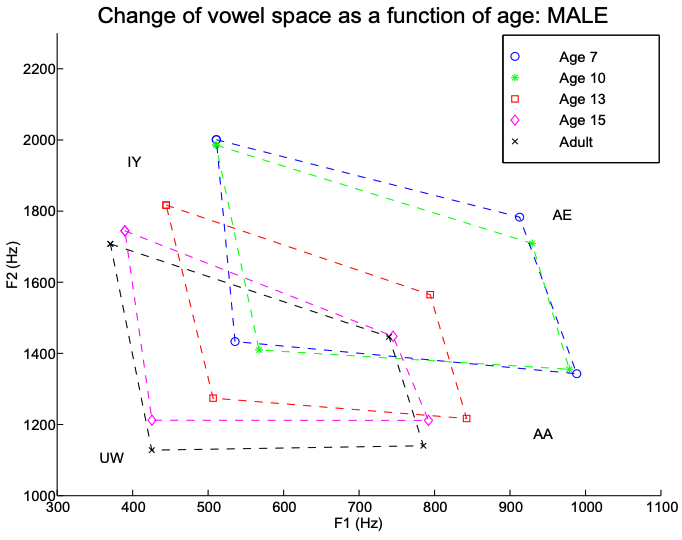
\includegraphics[width=0.48\textwidth]{imgs/f1f2children.png}}
\subfigure[Mean cepstral distance between the two repetitions of the same vowels]{\label{fig:intra_children}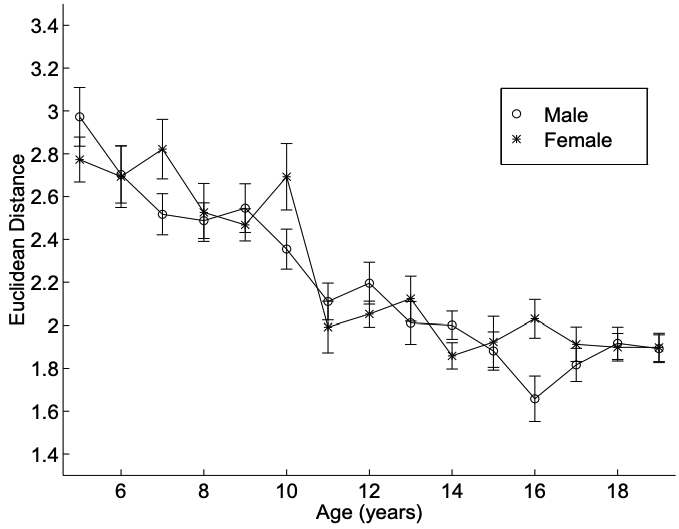
\includegraphics[width=0.48\textwidth]{imgs/intraspeakervariability.png}}
\caption{Formant and cepstral variability. Figures taken from \cite{reviewASRchildren}}
\end{figure}

\begin{figure}[ht]
\centering
\subfigure[Averaged-vowel duration across all vowels and subjects in each age group]{\label{fig:duration_vowel_children}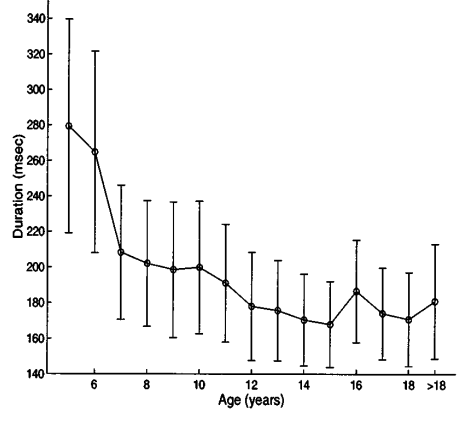
\includegraphics[width=0.48\textwidth]{imgs/children_vowel_duration.png}}
\subfigure[Within- and between-subject variations. The between-subject variation is reduced by a factor of 2.0]{\label{fig:intra_duration_children}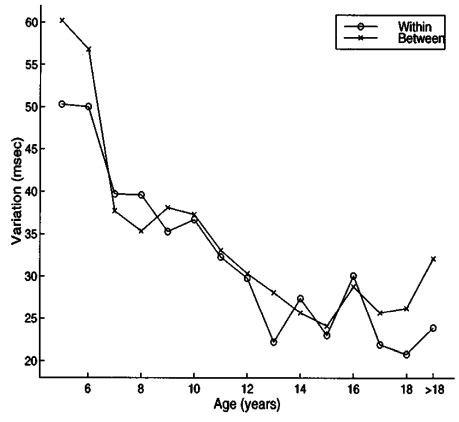
\includegraphics[width=0.48\textwidth]{imgs/Intra_inter_duration.png}}
\caption{Segmental duration variability. Figures taken from \cite{Acoustic_change_children}}
\end{figure}


In addition to inter-speaker variability, \cite{Acoustic_change_children} also highlight the fact that children's speech also exhibits intra-speaker variability, signifying that the speech produced by the same individual can exhibit variations. This variability arises from two primary sources. Firstly, as previously discussed, the acoustic characteristics of children can significantly differ at different ages due to the ongoing growth of their vocal apparatus.  Secondly, even at the same age, the same child may produce variable speech, even when articulating the same vowel. As depicted in Figure \ref{fig:intra_children}, the average cepstral distance between two repetitions of the same vowels by the same child tends to decrease with age, particularly after the age of 10. This reduction in intra-speaker variability is attributed to the progressive mastery of speech articulation components as children grow and mature their motor skills abilities. The decrease in cepstral distance suggests a more coherent and standardised articulation of vowels over time.

% Duration segments for children are longer
Segmental duration is another important aspect of human speech. A segment, as defined by Crystal \cite{segment_definition}, is: \textit{"Any discrete unit that can be identified, either physically or auditorily, in the stream of speech"}. These segmental durations could be of vowel or sentence duration. Vowel duration, in particular, is of significant importance in vowel discrimination. Research, as presented in \cite{Acoustic_change_children}, investigates how these characteristics change in children's speech. As demonstrated in Figure \ref{fig:duration_vowel_children}, the average vowels duration in children exhibits variations with age. On average, younger children tend to have longer vowel durations, resulting in a slower speaking rate. However, as children become more comfortable with the processes of speech production with age, vowel duration gradually decreases. Similarly to children frequency variations, segmental duration exhibits intra-speaker variability, as illustrated in Figure \ref{fig:intra_duration_children}.


% Conclusion on frequency challenges 
In conclusion, dealing with both intra- and inter-speaker variability in children's speech, particularly in those under the age of 15, poses a substantial challenge for developing high-performance speech processing models. Especially, this challenge is exacerbated in the context of children's \ac{ASR} where the age of the child is often unknown. In addition, the dynamic processes of the vocal tract growth, changes in linguistic knowledge and the maturation of control of speech apparatus occur simultaneously and overlap, making it considerably more challenging to accurately disentangle and model their effects. The intricate nature of children's speech, marked by intra and inter-speaker variations, underscores the necessity for sophisticated and adaptive models that can accommodate the unique characteristics of these speakers.



\subsection{Language and phonetic knowledge} %************************************************
\label{subsection:mispron}
% Intro on language and phonetic
Language is a complex and multifaceted system of communication that involves the use of symbols, such as words to convey meaning. It is a unique human ability and serves as a fundamental aspect of human cognition and social interactions. Linguists have identified five basic components of language \cite{moats2000speech}, including phonology (sounds), morphology (structure and construction of words) , semantics (meaning), syntax (grammar and sentence structure), and pragmatics (how language is used in context). It allows individuals to express thoughts, share information, and engage in social interactions. It is important to note that, languages vary across cultures and regions, exhibiting a rich diversity of sounds, structures, and expressions. Additionally, language can be spoken, written, or signed, and evolves over time. For children, the mastery of language is crucial milestone in their cognitive development. Futhermore, language plays a central role in shaping culture, identity, and the transmission of knowledge to them. The children's ability to use language develops with age, achieving adult capabilities around the age of 13, as indicated by \cite{Acoustic_change_children}. This progression enables the children to transition from producing simple sounds and words to generating more complex sounds and fully articulated sentences.

% Explain what are the main disfluency
During the process of language acquisition, children, constrained by their limited linguistic knowledge, often make pronunciation errors and encounter disfluencies \cite{language_children}. According to \cite{clark1977psychology}, these errors may include a variety of phenomena, such as:
\begin{itemize}
    \item \textbf{Substitution}:  Involves the inadvertent replacement of the correct pronunciation of an entire word with an alternative word.
    \item \textbf{Omission}:  Refers to the act of leaving out or neglecting a part of speech, a word, or a phrase that would typically be included in a grammatically correct or complete sentence.
    \item \textbf{Mispronunciation}:  Involves the act of pronouncing a part of a word incorrectly, deviating from the standard or expected pronunciation of this word.
    \item \textbf{Pause and Hesitation}: Entails temporary breaks or delays in speech during which a speaker might refrain from producing sound or articulate speech in a hesitant manner.
    \item \textbf{Filler and mumbling}:  Filler encompasses linguistic elements used during pauses or hesitations when a speaker needs time to think, including unintelligible sounds, words, or phrases without significant meaning. Mumbling is characterised by unclear or indistinct speech, often marked by low volume, unclear articulation, and imprecise pronunciation.
    \item \textbf{False-start}:  Refers to an instance where a speaker begins a sentence or a word and then stops abruptly before completing it. This interruption is often followed by a restart or a correction to articulate the intended message more accurately.
    \item \textbf{Sound-out}: Involves a pronunciation strategy in which a speaker articulates a word by pronouncing each sound or phoneme separately, rather than blending them together seamlessly.
\end{itemize}

% Give more example of disfluency over age
Potamianos and Narayanan's study \cite{language_children2} revealed significant insights into the variability and characteristics of children's linguistics. They found that inter-speaker variability is approximately twice as much as intra-speaker variability. Additionally, their research found that the rate of mispronunciations is twice as high for children aged 8 to 10 compared to those aged 11 to 14. Conversely, the trend is reversed for filler and pauses, where the older group exhibits a higher rate. Furthermore, younger children, of 8 to 10 years, tend to produce more false-starts and breathing.

% Explain that it is hard to model, that adaptation from adult because Children has different grammatical constructs 
In adult speech, pronunciation errors and disfluencies are also present, but their occurrences are typically lower than what is observed in the speech of children, as supported by studies such as \cite{Children_language_model,children_language_model2}. In addition, these studies used language models specifically trained on children's speech, demonstrating their advantages over the use of adult language models. This findings underscored the differences between children's and adults's linguistics, encompassing variations in grammatical structures as well as the presence of mispronunciations and disfluencies. Such insights are crucial for the development of effective language models tailored to the unique characteristics of children.


\subsection{Data scarcity}%****************************************************************
\label{section:data_scarcity}
% Data is key in this deep learning time
In recent years, the emergence of deep learning has brought significant advancements in the \ac{ASR} field. The combination of increased computational power and the availability of large datasets has played a pivotal role in these improvements. The success of deep learning is largely attributed to \ac{DNN}s, which can approximate complex non-linear functions. With the help of this capability, \ac{DNN} excels in capturing complex patterns and accurate representations of speech data. However, the efficacy of a \ac{DNN} in capturing speech patterns depends a lot on the availability of training data. Indeed, using large-size datasets is pivotal for enhancing the capabilities and generalisation of \ac{DNN}-based \ac{ASR} systems. Notably, top-performing \ac{ASR} systems like Whisper have been trained on  exceptionally large dataset, surpassing 680,000 hours of data collected from the web \cite{radford2023robust}. There is a noticeable trend in the speech research community towards the collection of larger datasets, exemplified by initiatives such as the LibriSpeech dataset, which comprises around 1,000 hours of speech \cite{librispeech}, and the GigaSpeech dataset, featuring 10,000 hours of speech \cite{chen2021gigaspeech}.

% Explain pb with children dataset
Unfortunatly, despite rare recent efforts to collect larger children datasets \cite{MyST,singakids,ahmed2021auskidtalk}, the majority of publicly available children corpora include fewer than fifty hours of speech. This is significantly less than a typical adult speech corpora, which usually contains hundreds or even thousands of hours of data. Furthermore, the majority of the accessible children's data are English corpus \cite{MyST,cmu,cslu,pf-star-british,ahmed2021auskidtalk}. However, English is a resource-rich pluricentric language which should be seen more as an exceptional case, rather than an average representative. A compilation of existing datasets containing children's speech will be presented in \ref{section:children_corpora}.

% Ethical problems
The scarcity of children's speech datasets availability can be partially attributed to a combination of ethical, legal, and technical challenges. Collecting speech data from children raises ethical concerns related to obtaining consent, ensuring privacy, and protecting minors. The heightened awareness of online safety and security concerns further complicates the creation and sharing of datasets that include children's speech, as there is a need to safeguard against potential misuse and ensure the anonymity of participants.
% Need of a diversity
Beyond ethical and legal considerations, technical challenges also play a role. Children's speech patterns, language development, and pronunciation can vary significantly across different age groups, as explained in previous sections, making it more challenging to create datasets that accurately represent the diversity of children's speech. Moreover, the resource-intensiveness of collecting high-quality speech data from children, which involves careful planning, recruitment efforts, and coordination with schools or parents, can further contribute to the limited availability of such datasets.
% age problem, school recording -> noise, attention span of the children
Finally, collecting speech data from children is a challenging and time-consuming task. Various factors can significantly impact the quality of the gathered speech. These include children's short attention spans, recording environments that might be noisy (such as classrooms), and the quality of the speech, which is highly dependent on the task at hand (reading tasks are generally more complex for children).

% explain that with data, a lot of problems can be solved
The importance of having a large database of children's speech to cover different variabilities has been emphasised in a study conducted by Liao in 2015 \cite{asr-google}. In this work, the researchers trained an \ac{ASR} model using a large in-house corpus of children's speech. Notably, this corpus was comparable in size to typical adult speech corpora. The result was the attainment of state-of-the-art performance by the \ac{ASR} model, even demonstrating competitiveness with adult speech recognition systems. This study underscores the crucial role of large-size and diverse children's speech datasets in developing robust and high-performance \ac{ASR} models tailored to the unique characteristics of children's speech.


\newpage
\section{Introduction to automatic speech recognition}%----------------------------------------------------------- ~11 pages
In this section, a brief historical overview of \ac{ASR} is presented, laying the foundation for a subsequent exploration of predominant trends and modules within \ac{ASR} systems. This comprehension is necessary for the following sections of this thesis. While not exhaustive, this overview provides essential insights, with certain topics falling beyond the scope of this thesis are intentionally omitted. For a more exhaustive understanding of \ac{ASR}, readers are encouraged to consult references such as \cite{benzeghiba2007automatic, karpagavalli2016review, arora2012automatic}. This section is structured as follows: Firstly, we present the historical evolution of \ac{ASR}, followed by an description of traditional HMM-based \ac{ASR} systems, succeeded by an explanation of the end-to-end paradigm. Concluding this section, a discussion on automatic speech recognition metrics is presented.

\subsection{A brief history of Automatic Speech Recognition}

\subsubsection{Early Days}

The origins of speech recognition technology can be traced back to the 1950s and 1960s, with initial projects focusing on isolated word recognition with a speaker-dependent system. One of the earliest project in this direction was the creation of a digit recogniser at Bell Telephone Laboratories in 1952. This recogniser demonstrated the automatic recognition of telephone-quality digits spoken at normal speech rates by a single adult male speaker, achieving an impressive accuracy of up to 99\%. The system relied on formant frequency approximations to recognise entire words. It is impotant to underscore that within this recogniser, there was an absence of explicit modeling of syllables, consonants, vowels, or any other sub-word units. In this recogniser, a word was treated as a single unit, which was then compared with ten standard digit patterns to find the best match. The recognition process first involved extracting two frequency ranges, below and above 900 \ac{Hz}. Motivated by the observation that these two frequency ranges approximately align with the frequencies of the first two formants in speech. Then, these formant approximations were plotted on a 2D-plot with a trace interruption period of 10ms. Finally, when presented with new audio, the system generated a new plot, compared it to the reference plots of the ten digits, and returned the closest match by computing the highest relative correlation coefficient. Figure \ref{Bell} illustrates an example of the 2D representation of the ten digits.


\begin{figure}[h]
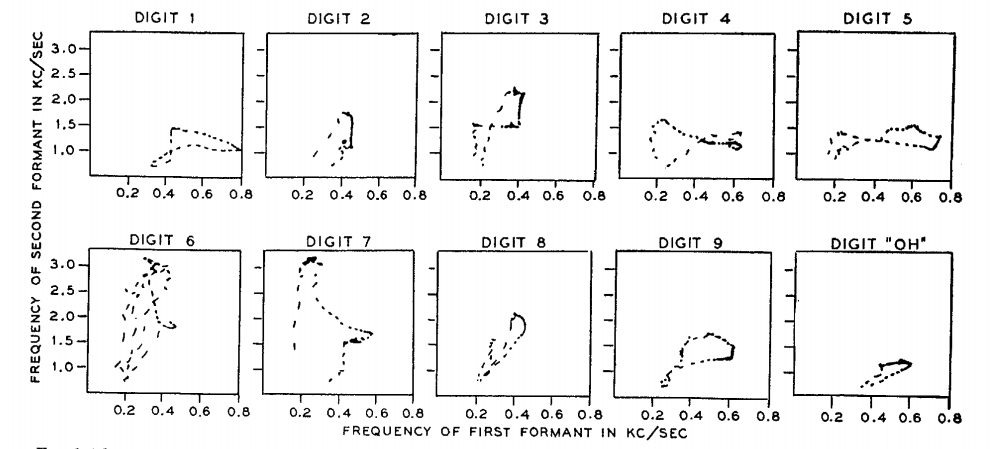
\includegraphics[width=\textwidth]{imgs/bell.png}
\caption{Example of a standard digit pattern from Davis et al. 1952}
\label{Bell}
\end{figure}


In 1962, IBM developed Shoebox, a device capable of recognising 16 spoken words, including the ten digits and command words such as "plus," "minus," and "total." This system employed a similar pattern-matching algorithm  to the one used in the Bell Telephone Laboratories's recogniser.


Nevertheless, extending such a system for a larger vocabulary would be impractical. Indeed, the template-matching approach necessitated saving each word representation on disk and comparing the unknown spoken word with all these representations. Therefore, when attempting to scale this approach to automatic large vocabulary recognition, issues of time and disk usage complexity emerged as a significant challenge. Furthermore, in order for the circuit to deliver an accuracy of the same range for a new speaker, a preliminary analysis of the speech of that individual and subsequent circuit adjustments were necessary. These limitations underscored the need for more scalable and adaptive approaches and led the field of automatic speech recognition to continued to evolve.



\subsubsection{The Speech Understanding Research program} 

In the early 1970s, subsequent to the initial success of pattern matching algorithms in single-word recognition, the Advanced Research Program Agency of the U.S. Department of Defense, ARPA, initiated funding for a five-year program called \ac{SUR}. The overarching goal of \ac{SUR} was to ``obtain a breakthrough in speech understanding capability that could then be used toward the development of practical man-machine communication system". Within the context of this program, four distinct research groups were funded: two from \ac{CMU}, one from Bolt Beranek and Newman Inc. (BBN Hwim), and the last one from \ac{SDC}. Each group was assigned a specific task, such as dealing with facts about ships, travel budget management, and document retrieval. The ultimate objective for each group was to create a system capable of recognising simple sentences within the context of their assigned task, using a vocabulary of 1,000 words and achieving a \ac{WER} of 10\% in a reasonable amount of time.


The realisation that the pattern-matching word identification strategy could not be directly applied to the challenge of sentence understanding prompted a redesign of the single-word identification system. In the first hand, one key recognition was that the acoustic characteristics of words can vary considerably based on the context of the sentence. The impracticality of storing each word and all its possible different variations on disk became apparent. Moreover, determining the boundaries of each word  was almost an impossible task, and even if these boundaries were identified, the pattern-matching computation, involving comparisons with each of the 1,000 stored words and all their possible variations, would be time-consuming and exceed the reasonable time requirement. Secondly, another crucial consideration in the redesign of the system was that the length of the spoken sentence is variable and unknown, in contrast to the relatively fixed length in single-word identification tasks.

To address these challenges, a shift was made to a smaller unit than the word for modeling speech -namely, phonemes. Phonemes are the smallest distinctive and meaningful units that compose speech. Each language is associated with a finite set of phonemes, typically fewer than 50, which can be combined to form words. This shift enabled a more efficient and flexible representation of speech, accommodating the variability in the pronunciation of words.

Among all the systems proposed in the project, the Harpy system implemented by Lowerre in 1976 by the \ac{CMU} team exhibited the best performances \cite{klatt1977review}. Harpy is a speaker-specific system that use a pattern-matching algorithm at the phoneme level instead of the word level. The system employs a set of 98 phonemes and diphones -a pair of consecutive phonemes- , encompassing pronunciations of all words, along with a graph compiling all accepted sentences using 15,000 states. When a new spoken utterance is provided to the system, it undergoes an initial processing phase, involving low-pass filtering at 5 k\ac{Hz}, digitisation at 10,000 samples per second, and computation of 14 linear prediction coefficients with a 10ms shift. To speed-up the decoding process, analogous adjacent acoustic segments are grouped together. Subsequently, these audio segments are compared against the 98 phoneme templates, and the system deduces the optimal path over the decoding graph. Figure \ref{harpy} provides an exempler of a decoding graph in the Harpy system.


\begin{figure}[h]
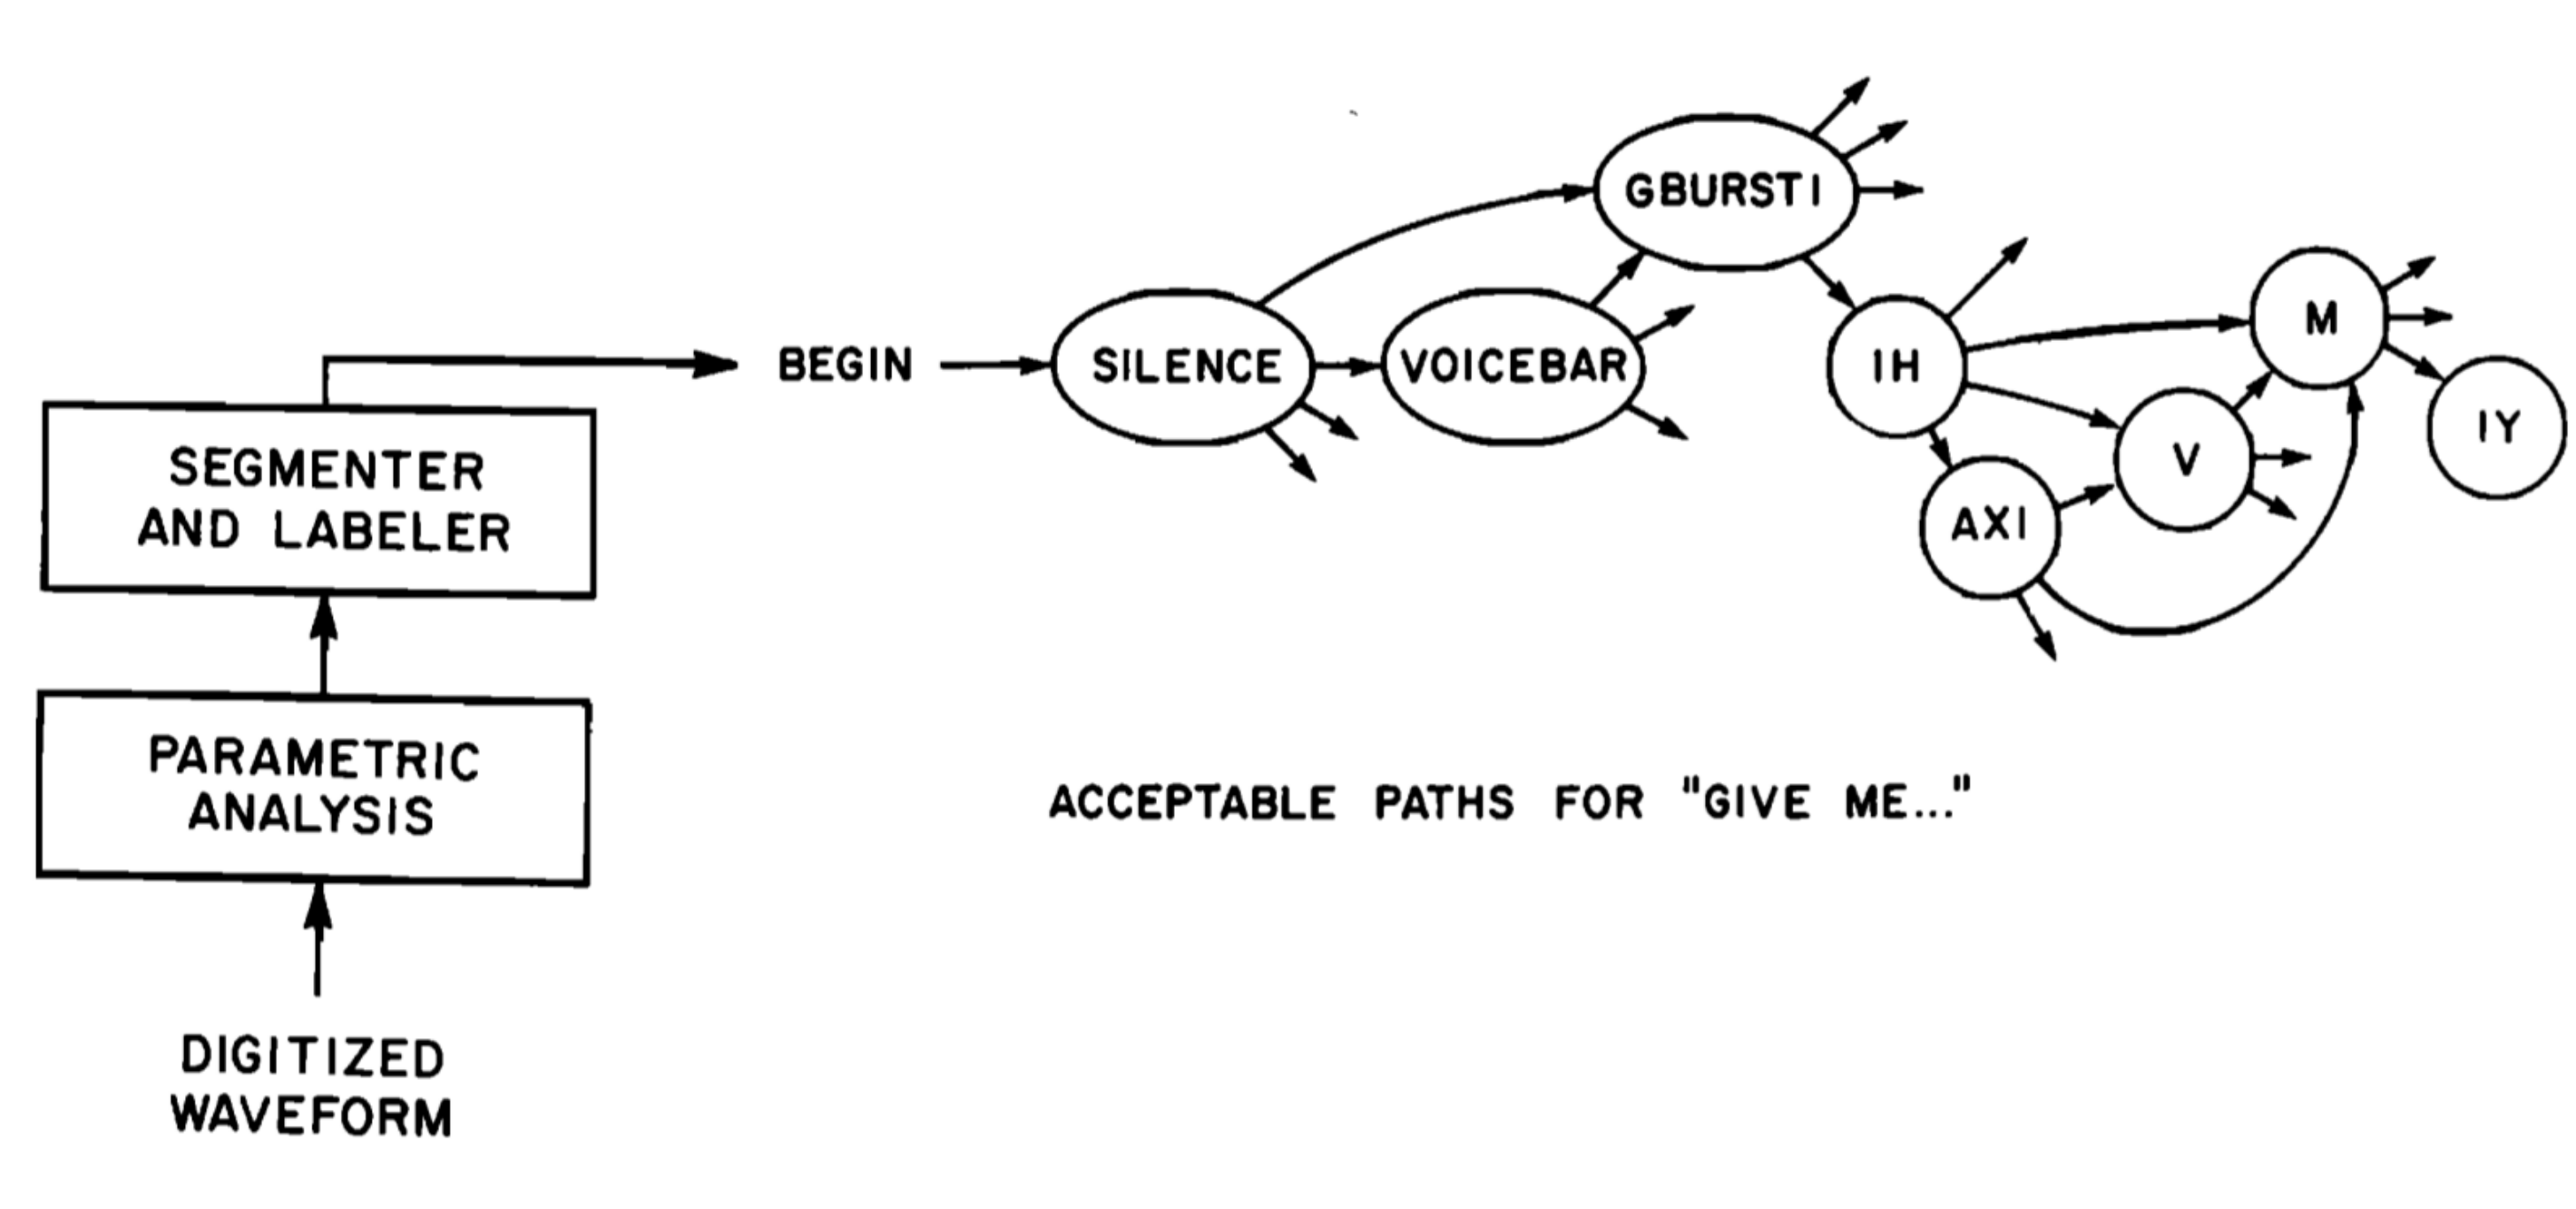
\includegraphics[width=\textwidth]{imgs/harpy.png}
\caption{Example of a decoding graph in the Harpy system for the sentence "GIVE ME" from \cite{klatt1977review}}
\label{harpy}
\end{figure}

Notwithstanding the achievements and success of the Harpy system, it has limitations that hinder its broader applicability. As a speaker-specific system, it requires tuning for each new speaker over the 98 phoneme templates. Additionally, the system is constrained to recognising a vocabulary of no more than 1,000 words and relies on a simple handcrafted grammar, making it less reliable for handling spontaneous speech. Moreover, the decoding time of the system falls short of real-time requirements. These constraints highlight the need for more generalisable and efficient speech recognition systems, especially for handling diverse speakers and spontaneous speech scenarios. Therefore, as research progressed, the limitations of pattern-matching based approaches became apparent. This realisation prompted the exploration of probabilistic modeling techniques, marking a shift towards more sophisticated and adaptable approaches in \ac{ASR}. 


\subsection{Traditional automatic speech recognition systems} % ~4 pages %************************
% HMM-DNN
\begin{figure}
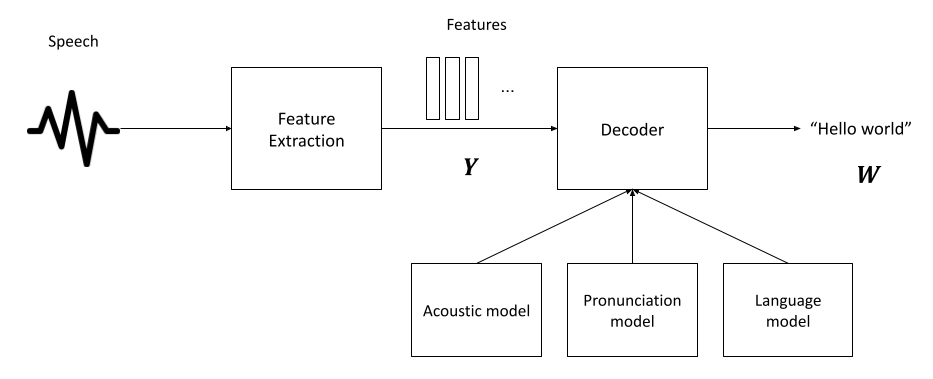
\includegraphics[width=\textwidth]{imgs/HMM-GMM_architecture.png}
\caption{Architecture of a HMM-based speech recognition system}
\label{HMM-GMM-model}
\end{figure}

%What are HMM
In the 1970s, the introduction of \acp{HMM} led to a paradigm shift in \ac{ASR} research, moving away from traditional pattern-matching methods towards statistical modelling \cite{first_asr}. Indeed, \acp{HMM} are particularly effective at capturing the sequential and temporal nature of speech. They assume that speech can be represented as a sequence of hidden states, each state corresponding to a distinct phonetic unit. \ac{HMM} models the transitions between these states and, at each state, generate observable acoustic features. The hidden aspect refers to the fact that the underlying states are not directly observed but inferred from the observable features. \acp{HMM} are particularly well suited to modelling speech dynamics, as they can represent the variability of speech sounds over time. In the context of \ac{ASR}, \acp{HMM} have been widely used to model phonemes, words or sub-word units.

%What are GMM
Building on this foundation, the 1980s saw the emergence of \acp{GMM}, which further enhanced the statistical modeling capabilities of \ac{ASR} \cite{htk_book}. \acp{GMM} allowed for a more flexible representation of the probability distributions underlying speech features.
\acp{GMM} are used to model the statistical distribution of acoustic features associated with each hidden state in an \ac{HMM}. Commonly, a system that uses both \ac{HMM} and \ac{GMM} is referred to as a \ac{HMM-GMM} framework. By using \ac{GMM}, they assume that the distribution of features can be approximated by a mixture of several Gaussian distributions. \ac{GMM} are versatile in capturing the variability of speech sounds, allowing a more flexible representation of the acoustic units. In \ac{ASR}, \acp{GMM} are commonly used to model the emission probabilities associated with each state in an \ac{HMM}. This means that given a particular state, the \ac{GMM} provides the likelihood of observing a specific set of acoustic features. By combining the temporal modeling capabilities of \acp{HMM} with the statistical representation power of \acp{GMM}, this framework effectively captures the complex relationship between acoustic features and phonetic units.

% What are statistical grammars
Finally, in the 1990s, statistical grammars also played a crucial role, providing a structured framework for incorporating linguistic informations into \ac{ASR} systems \cite{darpa1992}. Statistical grammars represent a category of grammars that integrate statistical information to characterise the probability of diverse linguistic structures. In contrast to traditional rule-based grammars, which articulate a language's syntax through explicit rules, statistical grammars adopt a data-driven methodology. They assign probabilities to various linguistic constructions based on observed frequencies within a designated corpus.

%What are DNN
The components illustrated in Figure \ref{HMM-GMM-model} represent the traditional \ac{ASR} pipeline. To this day, these components continue to form the core of modern \ac{HMM}-based \ac{ASR} systems. However, the recent evolution in the \ac{ASR} field has been marked by a significant shift from the \ac{GMM} to the adoption of \ac{DNN}. Driven by \ac{DNN} ability to effectively model complex patterns and hierarchies in speech data, \acp{DNN} have demonstrated superior performance, contributing to enhanced accuracy and efficiency in speech recognition systems \cite{hmm-dnn}. Called hybrid models, or \ac{HMM-DNN},by effectively combining both the strengths of \acp{HMM} and \acp{DNN}. A \ac{DNN} is a subtype of artificial neural networks consisting of multiple layers of interconnected neurons. These neurons, organised in layers, receive an input signals, and each connection between neurons is characterised by a weight that signifies its strength. In addition, each neuron is associated with a bias weight, provide an additional learnable parameter. During training, the network adjusts these weights and biases to minimise the difference between predicted and actual outputs, a process known as backpropagation. Moreover, a non-linear activation functions is placed within neurons, as it enables the network to models intricate, non-linear patterns of the data. The weights, biases and non-linearity allow \acp{DNN} to capture complex relationships and representations from the data,learning hierarchical features and abstracting information across multiple layers of the network.

%Math formulation
In this statistical framework, the continuous speech audio waveform is transformed into a sequence of fixed-size acoustic vectors, denoted as $\boldsymbol{X}=x_1,...,x_T$. The goal of the \ac{ASR} system is to determine the sequence of words, $\boldsymbol{w}=w_1,...,w_L$, that is most likely to have produced the observed acoustic vector sequence $\boldsymbol{X}$. This is formulated as finding the word sequence $\hat{w}$ that maximises the conditional probability $P(\boldsymbol{w}|X)$. More formally:

\begin{equation} \label{equation:asr_0}
    \boldsymbol{\hat{w}} = \argmax_{\boldsymbol{w}} \{P(\boldsymbol{w}|X)\}
\end{equation}
However, directly modeling the conditional probability $P(\boldsymbol{w}|X)$ can be challenging. Bayes' Rule offers a way to express this probability in terms of more manageable components, specifically by decomposing it into the product of the likelihood of the observed acoustic vector sequence given the word sequence $P(X|\boldsymbol{w})$ and the prior probability of the word sequence $P(\boldsymbol{w})$. Therefore, equation \ref{equation:asr_0} became:
\begin{equation}  \label{equation:asr}
    \hat{\boldsymbol{w}} = \argmax_{\boldsymbol{w}} \{\frac{P(X|\boldsymbol{w})P(\boldsymbol{w})}{P(X)}\} =\argmax_{\boldsymbol{w}} \{P(X|\boldsymbol{w})P(\boldsymbol{w})\}
\end{equation}
Here,  the likelihood $P(\boldsymbol{X}|\boldsymbol{w})$ is determined by the acoustic model component, capturing the probability of observing the acoustic vector sequence $\boldsymbol{X}$ given the word sequence $\boldsymbol{w}$. In parallel,  the prior probability $P(\boldsymbol{w})$ is determined by the language model component. The term $P(X)$ is not essential for determining the maximum probability and can be omitted in the context of finding the most likely word sequence. Subsequent sections will provide a more in-depth exploration of these distinct components and their processes.


% Feature extraction 
\subsubsection{Feature extraction}%*********************************************************
\label{subsection:features}

The feature extraction component plays a crucial role in capturing pertinent information about the linguistic content of speech. The efficacy of speech recognition systems is intricately tied to the quality of the extracted features. To this end, for each time step, the continuous waveform is transformed into a small fixed-size vector. A acceptable assumption is that speech is considered as stationary within the time span covered by a single vector. Consequently, feature vectors are typically computed at intervals of 10 milliseconds, often with a 25-millisecond overlapping window.

\begin{figure}
    \begin{center}
    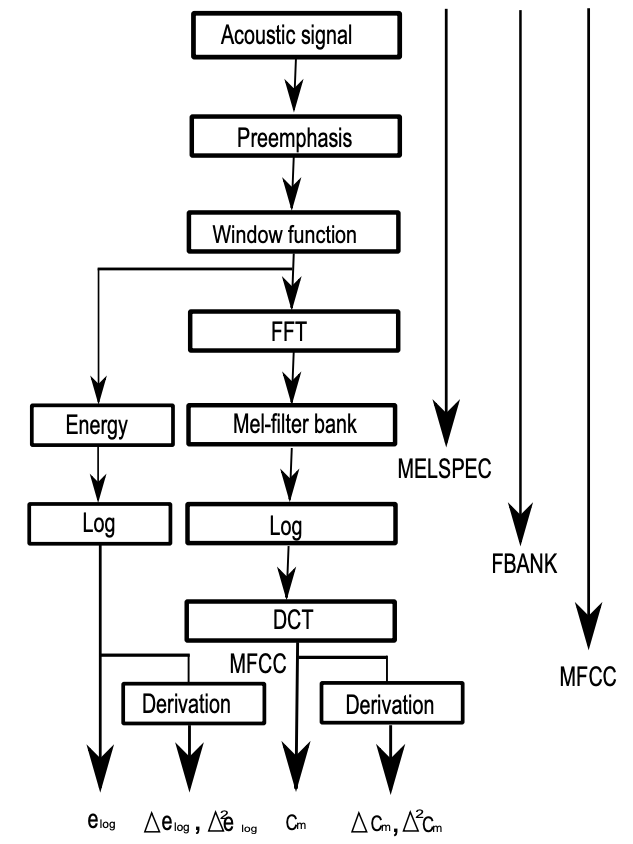
\includegraphics[scale=0.3]{imgs/features.png}
    \caption{Principal block scheme of main speech features for ASR: Melspec, fbanks and MFCC coefficients from \cite{kiktova2013comparison}}
    \label{feature_block}    
    \end{center}
\end{figure}

% MFCC
Within the domain of \ac{ASR}, a broad range of different acoustic features can be employed. However, in the context of \ac{HMM}-based models, the predominant features encompass  \ac{PLP}, Melspec, \ac{fbanks}, and\ac{MFCC}. However, \acp{MFCC} as introduced by Davis and Mermelstein \cite{mfcc}, stand as the predominant features in \ac{HMM-GMM} and \ac{HMM-DNN} architectures.
The process of extracting \acp{MFCC} typically involves several steps to capture essential information from the speech signal. First, a preemphasis filter is applied to the signal. Subsequently, the signal is segmented into frames, and a Hamming window with a duration of 25 milliseconds is applied to each frame. The frames are then transformed into the frequency domain using the discrete \ac{FFT}, resulting in the magnitude spectrum.
The next stage involves passing the magnitude spectrum through a bank of triangular-shaped filters. Extracting features at this point yields melspec features. The energy output from each filter is log-compressed, and concluding the extraction process at this stage results in fbanks features. Finally, \acp{MFCC} are obtained by transforming the filterbank features into the cepstral domain using the \ac{DCT} to decorrelate the energies obtained from the filterbanks. The representation of this extraction process is illustrated in Figure \ref{feature_block}.


%Delta features and concatenation

To incorporate information about the dynamics of the speech signal, the feature vector for each time step is augmented with the first and second-order derivatives, commonly denoted as $\Delta$ (Delta) and $\Delta\Delta$ (Delta-Delta), respectively. The first-order derivative coefficients, often referred to as $\Delta$ coefficients, are calculated by taking the difference between consecutive feature vectors. Mathematically, the $\Delta$ coefficients for a feature vector at time $t$ are computed as follows:
\begin{equation}
 \label{equation:delta}
    \Delta_i = \frac{\sum^{N}_{n=1}n(f_{i+n} - f_{i-n})}{2 \sum^N_{n=1}n^2} \\
\end{equation}
Here, $f_i$ represent the feature at the instant $i$.Typically, $n$ is set to 2, indicating that the first-order derivatives are calculated by considering the differences between the feature at the current time $t$ and its neighboring features at $t \pm 2$.The $\Delta\Delta$ coefficients, also written $\Delta^2$, represents the second-order derivatives and are computed in a similar manner as $\Delta$in equation \ref{equation:delta} by taking the difference between consecutive $\Delta$ coefficients instead of the spectral feature $f$. The concatenation of the first-order derivative ($\Delta$) and second-order derivative ($\Delta^2$) features with the spectral features is denoted as $x_i$. Mathematically, this concatenation can be expressed as follows:

\begin{align}
    \boldsymbol{x_i} = [f_i \qquad \Delta_i \qquad \Delta^{2}_i]
\end{align}
Here, $f_i$ represents the spectral feature at the instant $i$, $\Delta_i$ represents the first-order derivative feature at the same instant, and $\Delta^2_i$ represents the second-order derivative feature at the same instant. The resulting feature vector $x_i$ encapsulates information about the spectral content of the speech signal as well as its temporal dynamics, providing a more comprehensive representation for subsequent processing by the \ac{ASR} system, espacially the acoustic model.


% What is an Acoustic model
\subsubsection{Acoustic model}%****************************************************************
% There role and limitation of simple AM
The role of the \ac{AM} is to determine $P(\boldsymbol{X}|\boldsymbol{w})$. While employing a classifier such as \ac{GMM} models with one \ac{GMM} per phone is a straightforward approach, it tends to disregard the temporal dependencies inherent in speech, such as co-articulation. Indeed, accurately categorising each frame necessitates the consideration of not only the current frame but also its context, encompassing both previous and following frames. Additionally, there are acoustic differences at the beginning, middle, and end of each phone, further complicating the classification task. To address these concerns, the \ac{HMM} framework has been proposed as a solution \cite{Dragon_system}. \acp{HMM} offer temporal flexibility, incorporating concepts such as self-looping, and provide a well-understood framework with effective learning (Expectation Maximisation) and decoding (Viterbi) algorithms. 


\begin{figure}
    \begin{center}
    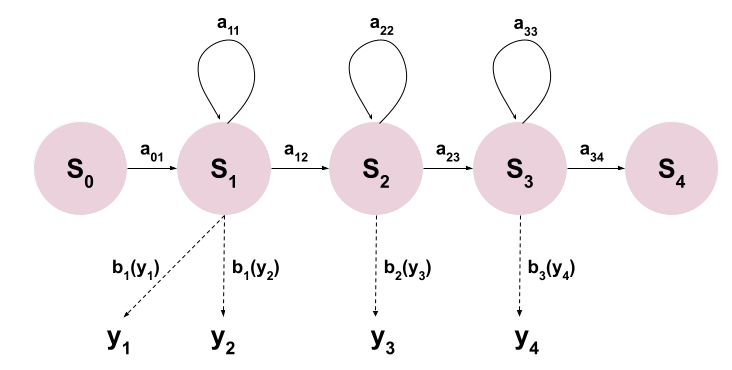
\includegraphics[scale=0.3]{imgs/HMM_monophone.png}
    \caption{Three-state Hidden Markov Model for modelling phones}
    \label{HMM_monophone}    
    \end{center}
\end{figure}
% Use of HMM and HMM-GMM
In the \ac{HMM} terminology, the observed variables, denoted as $y_i$, correspond to the acoustic features (e.g., speech signal), while the hidden variables are represented as states, denoted as $s_i$. The states are generated using a first-order Markov process, where the $i^{th}$ state $s_i$ depends solely on the previous state $s_{i-1}$. The transition from one state to another is determined by the transition probability $a_{ij}$. Upon entering a state $s_i$, an observation in the form of an acoustic vector is emitted, and this emission is modeled by the distribution $b_i(\cdot)$ associated with that state. Typically, this emission distribution is modeled by a \ac{GMM}. It is assumed that all observations are independent given the states that generated them. A fundamental configuration in \acp{HMM} for speech recognition involves a three-state model representing the beginning, middle, and end of a phoneme, along with an initial and final state. This model, known as a monophone \ac{HMM-GMM}, constitutes a basic unit for phonetic modeling. For example, since English has 44 phonemes \cite{bizzocchi2017many}, a monophone system on English will have 44 separate \ac{HMM-GMM}. However, due to the influence of co-articulation effects and the desire to capture phonetic variations based on context, more complex models, such as triphone systems, are employed \cite{schwartz1985context}. A triphone system aims to model each phoneme in its specific phonetic context, leading to a significantly larger number of required models.  Indeed, or a language with $N$ phonemes, there should be $N^3$ models to train. For example, in English, which has 44 phonemes, the total number of models would be  $44 * 44 * 44$ resulting in 85,184 models. To manage the computational complexity, these models are often clustered using decision trees \cite{bahl1991context}. This hierarchical clustering helps capture phonetic variations efficiently while working with limited available data.

% HMM-DNN
The concept of hybrid models gained prominence in the 1990s with the integration of \ac{MLP} as replacements for \acp{GMM} in the \ac{HMM-GMM} system \cite{bourlard2012connectionist,meinedo2003audimus}. Subsequently, the introduction of \acp{DNN}, which are \acp{MLP} with a large number of hidden layers, in 2012 marked a significant advancement in various \ac{ASR} tasks \cite{hmm-dnn}. The efficacy of \acp{DNN} lies in their capability to capture complex and highly non-linear relationships between inputs (e.g., audio features) and outputs (e.g., phoneme labels) due to the substantial number of parameters induced by the deep architecture.

However, the training of \ac{HMM-DNN} and \ac{HMM-GMM} models differs. Neural networks necessitate labeled data for training, which includes both input features and corresponding output labels (e.g., phoneme labels). Standard speech training data often lacks this detailed labeling, providing only audio waveforms and utterance transcriptions. Consequently, the training of \ac{HMM-DNN} models relies on alignments generated by an \ac{HMM-GMM}. Therefore, the training process involves initial flat-start monophone training with \ac{HMM-GMM}, followed by iterative steps into triphone training with more precise alignments. In consequence, the precision of the \ac{HMM-GMM} alignment directly impacts the efficacy of \ac{DNN} model training. As \ac{ASR} continues to advance, the integration of various \ac{DNN} architectures, including \acp{CNN} \cite{lang1990time}, \acp{LSTM} networks \cite{sak2014long}, and \acp{TDNN} \cite{waibel2013phoneme}, further refines the modeling of spatial and temporal relationships, laying the foundation for more sophisticated and context-aware speech recognition systems.

\subsubsection{Pronunciation model} %******************************************************
The pronunciation model in \ac{ASR}, often referred to as a dictionary or lexicon, plays a crucial role in establishing the correspondence between phonetic units, such as phonemes, and the respective words in the language. In \ac{ASR} systems, words are essentially comprised of phonetic segments, and the pronunciation model specifies how these segments combine to articulate the pronunciation of each word. This mapping takes the form of an entry where all possible words are associated with their corresponding sequence of phones. Examples of words along with their corresponding phonetic sequences are illustrated in Figure \ref{CMU_DICT}. Traditionally, this mapping is obtained manually, relying on phonetic and linguistic knowledge. It's noteworthy that a single word may have multiple pronunciations.

Furthermore, the integration of statistical \ac{G2P} tools \cite{g2p} augments the lexicon by facilitating the generation of pronunciations for words that may not be explicitly included in the dictionary.



\begin{figure}
    \begin{minipage}[t]{0.5\textwidth}
        \centering
        \begin{tabular}{ccc}
            \hline
            Phoneme & Example & Translation \\
            \hline
            AA & odd & AA D \\
            AE & at & AE T \\
            AH & hut & HH AH T \\
            AO & ought & AO T \\
            AW & cow & K AW \\
            AY & hide & HH AY D \\
            B & be & B IY \\
            CH & cheese & CH IY Z \\
            D & dee & D IY \\
            DH & thee & DH IY \\
            EH & Ed & EH D \\
            ER & hurt & HH ER T \\
            EY & ate & EY T \\
            F & fee & F IY \\
            G & green & G R IY N \\
            HH & he & HH IY \\
            IH & it & IH T \\
            IY & eat & IY T \\
            JH & gee & JH IY \\
            K & key & K IY \\
            \hline
        \end{tabular}
    \end{minipage}%
    \begin{minipage}[t]{0.5\textwidth}
        \centering
        \begin{tabular}{ccc}
            \hline
            Phoneme & Example & Translation \\
            \hline
            L & lee & L IY \\
            M & me & M IY \\
            N & knee & N IY \\
            NG & ping & P IH NG \\
            OW & oat & OW T \\
            OY & toy & T OY \\
            P & pee & P IY \\
            R & read & R IY D \\
            S & sea & S IY \\
            SH & she & SH IY \\
            T & tea & T IY \\
            TH & theta & TH EY T AH \\
            UH & hood & HH UH D \\
            UW & two & T UW \\
            V & vee & V IY \\
            W & we & W IY \\
            Y & yield & Y IY L D \\
            Z & zee & Z IY \\
            ZH & seizure & S IY ZH ER \\
            \hline
        \end{tabular}
    \end{minipage}
    \caption{Phoneme set and examples of CMU dictionary using 39 phonemes from \cite{weide1998carnegie}}
    \label{CMU_DICT}
\end{figure}


\subsubsection{Language model}%****************************************************************
% Role of language model
The \ac{LM}, often referred as grammar, holds a pivotal role in \ac{ASR}, responsible for determining the probability $P(\boldsymbol{w})$ of equation \ref{equation:asr}. Beyond its use in \ac{ASR}, the applications of language models extends into diverse fields including \ac{NLP} \cite{n-grams-NLP}, computational biology  \cite{n-grams-computational_biology}, and data compression \cite{n-gram-compression}. The two most successful approaches to language modeling widely adopted in \ac{ASR} are, respectively, statistical methods and models based on deep learning. 


% N-grams
Statistical \acp{LM} rely on traditional techniques like \ac{HMM} and N-grams. N-grams, which are the simplest approach for language modelling, estimate the likelihood of the next word based on the context of the preceding $n$ words as follows:
\begin{equation}
    P(\boldsymbol{w})= P(w_1 , w_2 ,\dots,w_L)  =\prod_{i=1}^L P(w_i| w_{i-n} , \dots,w_{i-1}  )
\end{equation}
The granularity of context varies from the case when $n=1$, the 1-gram -or unigram (considering each word independently) to higher-order $n$-grams that incorporate more extensive context for enhanced accuracy. The unigram model would be defined as follows:
\begin{equation}
    P(\boldsymbol{w})=P(w_1, w_2,\dots,w_L )  = \prod_{i=1}^L P(w_i)
\end{equation}
Despite the evident advantages of employing a larger $n$ for enhanced contextual information in language modeling, practical considerations and computational limitations often impose constraints on the choice of $n$ in real-world \ac{ASR} applications. The escalating combinational complexity associated with higher $n$ values becomes computationally demanding, presenting challenges for efficient processing, storage, and training. As a result, the majority of \ac{ASR} applications typically use trigrams or 4-grams, striking a balance between contextual accuracy and computational feasibility.

Furthermore, determining the start of sequence probability precisely introduces intricacies, especially with larger $n$-grams. Additionally, the reliance on training data poses a notable limitation for $n$-grams, particularly in estimating the likelihood of unseen words. This deficiency becomes apparent when facing vocabulary expansion or encountering out-of-vocabulary terms, necessitating specific techniques such as smoothing to address these challenges.\cite{n-grams-smoothing}.

% Deep learning based LM
In contrast, deep learning-based \acp{LM} have opened up a new era, employing neural networks with complex architectures to achieve remarkable modeling capabilities. Unlike traditional n-grams, these models demonstrate a high degree of flexibility, ease training and do not require as many resources as n-grams to be efficient. Recent advances in language modeling, exemplified by state-of-the-art models such as \ac{BERT} \cite{Bert} or \ac{GPT} \cite{brown2020language}, are built on deep learning networks.


A key factor contributing to the success of deep learning language models is the incorporation of attention mechanisms. Unlike the limited contextual awareness of n-grams, attention mechanisms allocate varying degrees of importance to different words within a sentence. This approach enables the model to focus more on crucial elements, capturing intricate dependencies and semantic information that contribute to a more accurate language representation. The attention mechanism's ability to discern and prioritise important words enhances the overall performance and effectiveness of deep learning language models.


\subsubsection{Decoder}%**********************************************************************

In the context of \ac{ASR}, the decoder role is to use the language, acoustic, and pronunciation models to determine the most likely word sequence, denoted as $\boldsymbol{\hat{w}}$, given a corresponding sequence of acoustic features, denoted as $\boldsymbol{Y}$ (as refered in equation \ref{equation:asr_0}). This is achieved by employing dynamic programming to search through all potential sequences. Notably, the Viterbi algorithm \cite{viterbi_decoder}, are instrumental in efficiently solving this decoding problem. However, in practical applications, a direct implementation of the Viterbi algorithm becomes challenging, especially for continuous speech, where considerations such as model topology, language model constraints, and computational constraints must be taken into account. N-gram language models and cross-word triphone contexts further complicate the search space. To address these challenges, various approaches have emerged. 

One approach involves constraining the search space by maintaining multiple hypotheses in parallel \cite{valtchev1994novel} or dynamically expanding it as the search progresses \cite{aubert1995large}. Another alternative is to use beam search where the idea is to prune search path which are unlikely to successed. More recently, recent advancements in \ac{WFST} technology offer a comprehensive solution by integrating all necessary information, including acoustic models, pronunciation, and language model probabilities, into a single, highly optimised network \cite{mohri1997finite,caseiro2002using}. This approach provides both flexibility and efficiency, making it valuable for both \ac{ASR} research and practical applications. As demonstrated by the Kaldi speech recognition toolkit \cite{kaldi}, which  stands out as a widely adopted toolkit that leverages \acp{WFST} for decoding. 

Although decoders are primarily designed to find the best solution to the aforementioned probability computation in equatio \ref{equation:asr_0}, they can also generate the N-best set of hypotheses. This capability enables multiple passes over the data without incurring the computational expense of repeatedly solving the probability computation from scratch. The word lattice \cite{richardson1995lattice} serves as a convenient structure for storing these hypotheses, consisting of nodes representing points in time and spanning arcs representing word hypotheses.
Word lattices offer remarkable flexibility, allowing for rescoring by using them as input recognition networks. Furthermore, they can be expanded to facilitate rescoring by a higher-order language model.


\newpage
\subsection{End-to-end automatic speech recognition} % 1-2 pages%*********************
\label{section:SOTAE2E}
\begin{figure}
    \centering
    
\includegraphics[width=\textwidth]{imgs/End2End_architeccture.png}
    \caption{Architecture of an end-to-end speech recognition system}
    \label{fig:e2e_archi}
\end{figure}
% Intro on E2E
 End-to-end speech recognition signifies a transformative paradigm in the field, presenting a streamlined and holistic approach compared to traditional \acp{HMM}-based systems. In contrast to conventional modular systems that incorporate distinct acoustic, pronunciation, and language models, end-to-end architectures propose to simplify the \ac{ASR} process by directly map input audio signals to transcriptions within a single neural network model as illustrated in \ref{fig:e2e_archi}. Indeed, One of the key disadvantages of hybrid models is the factorized training of all modules independently, which can lead to error accumulation and mismatches between the different components. Therefore end-to-end strategy simplifies the overall system design, eliminating the requirement for pre-aligned training data and post-processing of outputs, thereby fostering a more data-driven and automatic learning process.
 In this paradigm, word-level transcriptions are transformed into character-level transcriptions. Considering the sequence of fixed-size acoustic vectors $\boldsymbol{X}=x_1,...,x_T$ and the corresponding character sequence $\boldsymbol{Y}=y_1,...,y_N$, where $T$ and $N$ represent the numbers of frames and the length of the character sequence respectively, the objective of end-to-end models is to learn the conditional probability of the character $y_i$ given the input $\boldsymbol{X}$ and the preceding output $y_{<i}$:

 \begin{equation}
     P(Y|X) = \prod_{i=1}^{N}P(y_i | X,y_{<i})
 \end{equation}

 In recent years, with the growing interest in the end-to-end \ac{ASR} paradigm, these systems have demonstrated increasing performances. Particularly, in scenarios where a large amount of labelled training data is available,  end-to-end systems have demonstrated comparable or even superior performance compared to traditional \ac{HMM}-based systems across various \ac{ASR} datasets \cite{hannun2014deep,hmmvse2e}. However, despite its promising results, end-to-end speech recognition faces a several challenges. Most importantly, these systems require a large corpus of training data to operate effectively. In the absence of such a corpus, the model may struggle to perform correctly \cite{hmm-end2end}. In addition, handling rare or out-of-vocabulary words remains a significant challenge. Finally, the generalisation across new acoustic conditions of the model can be issue. Therefore, there is a need of research on end-to-end speech recognition, particularly to simplify the end-to-end design, training, and robustness of these speech recognition systems.
 
 The overall struture of end-to-end systems depicted in figure \ref{fig:e2e_archi} highlight the integration of acoustic model, pronunciation model, and language model into a single neural network in end-to-end architectures. Nevertheless, feature extraction stage remains identical to traditional \ac{ASR} systems. In end-to-end systems, the most commonly employed fixed-size acoustic features are filterbanks. Motivated by the higher flexibility they provide when capturing relevant information from the speech signal compared to \acp{MFCC}.

 Transitioning to the end-to-end paradigm has necessitated the development of new training approaches. Indeed, training an end-to-end model differs significantly from training traditional \ac{HMM}-based systems. Notably, two training procedures have emerged in the literature of end-to-end \ac{ASR}: Connectionist Temporal Classification and sequence-to-sequence architectures. Each approach comes with its own distinct features and advantages, and the subsequent sections offer a more in-depth exploration of these two methodologies. It is worth mentioning that while these are distinct methods that can function independently, they can also be employed in conjunction.

 
 \subsubsection{Connectionist Temporal Classification}
 The first step towards end-to-end automatic speech recognition was made with the introduction of the \ac{CTC} objective function, introduced by Grave et al. \cite{First_End2End}. The main innovation of \ac{CTC} is that it eliminates the need for pre-segmented training data, enabling the model to automatically learn the alignments between the $N$ input speech frame $\boldsymbol{X}$ and the output sequence of $T$ phones $\boldsymbol{Y}$ if $N \leq T$, representing a departure from the traditional HMM-based models

 To this end, the \ac{CTC} objective function consists of two essential sub-processes: path probability calculation and path aggregation. Consider $\mathcal{V}$ as the set of possible paths of phone-label sequences of length $T$, and let $p^t_k$ denote the probability of observing the label $k$ at time $t$. It is noteworthy that \ac{CTC} necessitates the length of the label sequence $Y$ to be equal to $T$. To address any length difference between $N$ and $T$, a blank label ``-'' is introduced, representing the probability of observing no label. 
 
 First, the path probability calculation involves computing the conditional probability of any path $\pi \in \mathcal{V}$ given the observed acoustic features $\boldsymbol{X}$.Mathematically, this is expressed as:
 \begin{equation}
    p(\pi|X) = \prod_{t=1}^{T}p_{\pi_t}^{t} , \forall \pi \in \mathcal{V}
\end{equation}
 Where $\pi_t$ denotes the label at time $t$ in sequence path $\pi$. Considering all possible paths and their respective probabilities is crucial, but direct computation becomes infeasible due to the exponential number of potential paths.
 
 To address the computational challenges, the path aggregation step comes into play. Its purpose is to sum the probabilities of paths that correspond to the same label sequence $\boldsymbol{Y}$ by marginalizing over all possible paths. The path aggregation also merge the same contiguous labels and deletes the blank label. For example two different paths ``b-ii-r-d'' and ``b-i-r-dd'' becomes ``bird''. This is mathematically represented as:
\begin{equation}
    p(Y|X) = \sum_{\pi \in \theta_Y}p(\pi|X)
\end{equation}
Where $\theta_Y$ is a subset of $\mathcal{V}$ of all possible path $\pi$ corresponding, after aggregation, to the label sequence $Y$.

\subsubsection{Sequence to sequence}
%LAS attention mechanism and seq2seq
The \ac{Seq2seq} architecture, initially proposed by Sutskever for machine translation \cite{sutskever2014sequence} and stands as a important paradigm of end-to-end \ac{ASR} systems. The original context of its application was for machine translation tasks where a word sequences were translated from one language to another. The inherent challenge lies in the differing lengths of input and output sequences. However, this architectural framework, especially with the integration of attention mechanisms \cite{bahdanau2014neural}, has showcased remarkable versatility, extending its efficacy across diverse applications such as image captioning \cite{seq2seq_imagecaption}, conversational modeling \cite{vinyals2015neural}, text summarisation \cite{nallapati2016abstractive}, and \ac{ASR} \cite{dong2018speech}.

The core components of a standard \ac{Seq2seq} model consist of an encoder and a decoder. The encoder processes input sequences of variable length, transforming them into a sequence of vectors often denoted as the "internal state" or "hidden representation." This sequence of vectors encapsulates the crucial information extracted from the input features. Subsequently, the decoder uses this sequence of vector representation to generate an output sequence of tokens iteratively. Mathematically expressed as:
\begin{equation}
    p(y_1,...,y_T) = \prod_{i=1}^{T} p(y_i| y_0,...y_{i-1}, f(H))
\end{equation}
where $f(H)$ represents a function of the encoder's output $H = (h_1, ..., h_N)$. Notably, in \ac{Seq2seq} models incorporating attention mechanisms, $f(H)$ includes attention to selectively focus on relevant segments within $H$ for predicting the current target token. The \ac{Seq2seq} objective function is formulated to train the model by maximizing the conditional probability of generating the target sequence given the input sequence using \ac{NLL} loss or \ac{CE} loss.

A significant difference from \ac{CTC}-based models lies in the fact that \ac{Seq2seq} models do not make independent assumptions about output labels. Instead, they directly model the conditional probability of each target token given the preceding tokens in the output sequence and the encoder's output. This end-to-end approach empowers \ac{Seq2seq} models to handle sequences of varying lengths, making them particularly advantageous for tasks, like speech recognition, where precise alignment between input and output is challenging.


\subsection{Automatic Speech Recognition metrics}%**********************************************************************
% What is WER
In the domain of \ac{ASR}, metrics serve as indispensable tools for assessing the accuracy and effectiveness of systems. These metrics provide quantitative evaluations that act as a crucial benchmark, enabling researchers, developers, and engineers to objectively measure the performance of their \ac{ASR} models. The evaluation process of \ac{ASR} systems involves a meticulous comparison between system-generated transcriptions and reference transcriptions. Among these metrics, \ac{WER} is the most commonly used for assessing speech-to-text systems. The ASR system's output word sequence is matched with a reference transcription, and the number of \ac{S}, \ac{D}, and \ac{I} are summed. As a result, \ac{WER} is calculated as follows:
\begin{equation}
    WER = \frac{S  + D +I}{N} \times 100
\end{equation}
Where $N$ is the total number of words in the reference transcription. As a result, a lower \ac{WER} score is indicative of better system performance. The computation of \ac{WER} is based on the Levenshtein distance, operating at the word level rather than the phoneme level. The primary goal is to quantify the dissimilarity between the \ac{ASR} system's output and the reference transcription. Notably, a \ac{WER} score greater than 100\% can be attained when the number of mistakes surpasses $N$, while a score of 0\% is the minimum achievable when there are no errors in the \ac{ASR} hypothesis compared to the reference.

% Give example of ASR benchmarks
State-of-the-art \ac{ASR} systems developed by leading research institutions and companies have achieved \ac{WER} scores ranging from around 4.3\%  to 8.13\% on well resourced benchmark datasets such as the Switchboard corpus for conversational speech recognition \cite{tuske2021limit} and the French subset of the read speech Common voice dataset \cite{bermuth2021scribosermo} respectively. However,it is important to note that \ac{WER} scores can be task-specific, and achieving high \ac{WER} scores, especially in challenging conditions or for certain languages and accents, such as 38.9\% for the CHiMIE-6, a low resource noise speech dataset \cite{chan2021speechstew}.

Beyond \ac{WER}, there exist other metrics derived from the same fundamental equation but operating at different levels of transcription. Examples include \ac{PER} for languages based on phonemes and \ac{CER} which operates on character instead of word. These metrics provide a nuanced evaluation by concentrating on specific linguistic units, contributing to a comprehensive assessment of \ac{ASR} system performance in diverse contexts.

\newpage
\section{Children automatic speech recognition} % ~6-10 pages%*******************************
% But people try to tackle children's speech challenges ->
Addressing the challenges highlighted in Section \ref{section:Children_seepch_challenges} has prompted diverse initiatives across various segments of the \ac{ASR} pipeline. This involves exploring improvements at the feature level, with the development of novel extraction techniques and adaptations. Data augmentation strategies have been employed to enrich training datasets, offering the model exposure to a more diverse range of children speech patterns.  Modifications in annotation detail have been explored, refining the labeling process to better capture the nuances of children's speech.

% Describe the following sections
Beyond feature-level interventions, advancements in acoustic model structures have been pursued. This involves exploring new architectures and refining existing ones to better accommodate the characteristics of children's speech. In addition, innovative training procedures have been introduced to optimise model learning from the available data.

This section reviews state-of-the-art for each of these aspects in more detail. Following this comprehensive review, we will identify and delineate the specific approaches that emerge as promising or particularly impactful for addressing the challenges associated with children's  \ac{ASR}. These identified approaches will serve as the focal points for the subsequent phases of the thesis.
 
% Main focus on AM even though some work have been done in other part of HMM-based components
\subsection{Feature extraction stage}%*******************************
Feature extraction stage is critical for identifying relevant speech signal components for both traditional and end-to-end \ac{ASR}. This phase is characterised by the intentional elimination of speaker-dependent attributes, such as fundamental frequency, while simultaneously preserving the integrity of phoneme-dependent characteristics, notably exemplified by formant frequencies as described in section \ref{subsection:features}. In the context of children's speech recognition, the acoustic characteristics pose unique challenges, including close fundamental frequency and formant values, as well as phonetic class overlap due to formant variability. In addition, studies by \cite{ghai2009exploring,ghai2011addressing} demonstrated that in mel-filterbank-based cepstral features commonly used in the \ac{ASR} field, the acoustic mismatch is exacerbated by insufficient smoothing of pitch-dependent distortion present for child speakers To tackle these challenges, various strategies have been proposed to enhance acoustic features for children's speech, encompassing new feature extraction, feature adaptation, and the concatenation of new features.


% FEATURE EXTRACTION
%\subsubsection{Feature extraction}
%PLP features
An early step in the direction of better feature extraction for children was the introduction of \ac{PLP} features in 1990 by Hermansky \cite{Hermansky1990PerceptualLP}. Indeed, \ac{PLP} features demonstrated  a more accurate representation of formants in children's speech.  An additional strategy employed was the use of binary-weighting of \acp{MFCC}. This approach involves truncating some of the higher coefficients to remove those with non-sufficient smoothing, as proposed by \cite{ghai2009exploring}. The objective is to refine the representation of \acp{MFCC} by selectively retaining non-distorted coefficients. Furthermore, Gamma-tone filterbanks were employed to wrap the spectrum on a different scale, aiming to decrease variance compared to mel-filterbank features \cite{shahnawazuddin2023gammatone}.

% Extract features from raw speech directly
More recently, there has been a shift in the feature extraction stage from a hand-crafted approach to a data-driven strategy, focusing on learning relevant features directly from the raw speech signal. This approach, initially proposed by \cite{feat_ext_from_raw}, is motivated by the understanding that hand-crafted features are often based on the analysis of adult speech, and they may not be optimally suited for the acoustic variability present in children's speech. In the study conducted by \cite{feat_ext_from_raw}, data-driven feature extraction was performed using \ac{CNN}-based models. The results indicated that the features learned in a data-driven manner outperformed standard hand-crafted features, emphasising the potential benefits of adapting feature extraction to the specific characteristics of children's speech. Another similar approach was proposed by \cite{sincnet_adapt}, where the convolutional layers of the feature extractor were replaced by SincNet layers \cite{Sincnet}. SincNet use rectangular band-pass filters instead of the standard \ac{CNN} filters, enabling a reduction in the number of parameters required for raw waveform modeling. Additionally, this approach involves restricting the filter functions rather than having to learn every tap of each filter. 


% VTLN - Talk about limitation of VTLN
An alternative approach to mitigate the acoustic variability in children's speech involves working directly with adult features and adapting them to reduce children's acoustic variability. One common technique for this purpose is\ac{VTLN}, which has been widely employed to normalize spectral features into a canonical space \cite{VTLN, VTLN2}. Research conducted using \ac{VTLN} indicates a higher recognition rate when the \ac{ASR} system is trained with adult speech and subsequently tested with children's speech \cite{claus2013survey,potamianos1997automatic}. Indeed, \cite{potamianos1997combining} showed a strong relationship between the optimal warping factor and the age of speakers. \ac{VTLN} is typically applied as a front-end processing step at the end of the feature extraction. The \ac{VTLN} process involves stretching or compressing the frequency axis of the spectrum accoding on a warping function. This process leads to a normalisation of the spectral representation, reducing the impact of speaker variance. Nevertheless, it is important to acknowledge that recognition results achieved with \ac{VTLN} compensation alone may still be sub-optimal. This is attributable to the presence of various factors, extending beyond variations in vocal tract length, that contribute to the distinct characteristics between adult and children's speech.
%f0 normlization and pitch normalized & Speaking rate adaptation
In addition to directly adaptating speech feature, researchers have explored the normalisation of specific aspects of children's speech to better align with adult speech characteristics. Several studies investigated the use of pitch normalisation to reduce the spectral mismatch between children's and adult's speech \cite{f0norm,pitchnorm,pitch_adapt_norm, shahnawazuddin2023gammatone},  while other direclty normalised formant values \cite{formant_norm,kumar2023effect}. Furthermore, adapting speaking rate through time-scale modification approaches has been investigated \cite{speaking_rate}. Children's speech is typically slower than that of adults, and adjusting the speaking rate can aid in creating a more consistent representation for \ac{ASR} models.

% Machine learning adaptation
Moreover, in line with the trend of transitioning from knowledge-based to data-driven, some recent studies have explored data-driven feature adaptation methods using deep learning approaches. For instance, studies like \cite{adversarial-adapt1,adversarial-adapt2} employed adversarial multi-task learning to generate age-invariant features. The goal is to minimise the acoustic mismatch between adult and children's speech by leveraging adversarial training techniques. Adversarial training introduces a form of competition between neural networks, with one network generating features used by the \ac{ASR} and another network attempting to distinguish between the adapted children's features and the real adult's features. This adversarial approach aims to extract features that are less influenced by age-related variations, contributing to improved model generalisation across different age groups.

%\subsubsection{Additional features}
In addition to feature extraction and feature-level adaptation, certain studies have emphasised the efficacy of appending supplementary information to the acoustic features. For instance, it is a common practice to concatenate speaker embeddings, such as i-vectors \cite{ivector}, with acoustic features to achieve a more speaker-independent model \cite{shivakumar2020transfer}. Speaker embeddings are compact, fixed-size representations of the features of a speaker's voice derived from their speech signals. Concatenating speaker embeddings with the acoustic features enables the model to be more robust to speaker variability, as it incorporates an explicit representation of it. Similarly, both \cite{prosody_feat,kadyan2023prosody} proposed to  concatenate various prosodic features, including loudness, voice intensity, and voice probability, with standard acoustic features. This approach has demonstrated success in reducing inter-speaker variances and enhancing discrimination between phoneme classes.


\subsection{Pronunciation and language model}
%\subsection{Detail of the annotation}
% age dependent subset
The conventional information provided in speech corpora typically includes audio signals, corresponding text transcriptions, and anonymized speaker identifiers. However, augmenting this data with additional information holds promise for improving children's speech recognition systems. One pertinent aspect is incorporating the speaker's age, a critical factor, as described in section \ref{section:Children_seepch_challenges}, that could facilitate the development of age-dependent \ac{ASR} systems \cite{linguistic-children, gale2019improving}. 
% Sub-word and personalised lexicon
Moreover, annotating at the sub-word level, rather than the word level, has demonstrated increased performances, particularly in addressing challenges such as mispronunciations or hesitations \cite{subwords}. This approach enhances robustness by focusing on smaller linguistic units allowing more flexibility. Another strategy involves the implementation of children specific pronunciation model, as illustrated in \cite{pronunciation,pronunciation2}. These lexicons are specifically created to handle pronunciation divergences from canonical adult patterns with knowledge based children patterns.
% LM for children
Finally, the creation of language models explicitly tailored for children's speech can further improve the recognition accuracy \cite{children_language_model2,Children_language_model}. These models capture the linguistic nuances and variations intrinsic to children's language. The integration of these strategies collectively contributes to the development of more effective and adaptive \ac{ASR} systems for children.

\subsection{Design of acoustic models}%*******************************
The acoustic model is a pivotal component in \ac{ASR} for children's speech, as acoustic variability significantly affects the degradation of recognition accuracy compared to linguistic variability. Consequently, the design of the acoustic model is crucial for ensuring robustness to the specific characteristics of children's speech.

Initially, the transition from monophone to triphone \ac{HMM-GMM} models helped improve performance by capturing coarticulation effects \cite{potamianos1997automatic,language_children2}. A literature review \cite{bhardwaj2022automatic} indicates that much of the research on children's \ac{ASR} is based on \ac{HMM-GMM} models \cite{bhardwaj2022automatic}. However, acoustic models for children naturally align with the latest advancements in acoustic modeling for adults. Therefore, the design transitions from \ac{HMM-GMM} to \ac{HMM-DNN}, as proposed by \cite{TFchildren}.


The limitations of traditional fully connected neural networks in providing sufficient contextual informations prompted their replacement by \ac{TDNN} layers, as proposed in \cite{tdnn}. \acp{TDNN} function similarly to one-dimensional convolutional neural networks. At each time step, both the current time-step frame and its corresponding left and right context are considered, in contrast to traditional \acp{DNN} that focus solely on the current time step. To further improve the model's capacity to capture extensive contextual information, multiple layers of \ac{TDNN} can be used. In addition, motivated by the large overlaps between neighboring input context sub-sampling was introduce. Sub-sampling involves allowing gaps between frames in the context window. 
While \ac{TDNN} were demonstrated as successful desing for children \ac{ASR} \cite{kumar2020leveraging}, they were quickly replaced by \ac{TDNN-F}. Indeed, \ac{TDNN-F} were introduced as an improvement of regular \ac{TDNN} \cite{TDNN-F} by decomposing the weight matrix using \ac{SVD}. A more detailed explanation of \ac{TDNN} and \ac{TDNN-F} will be provided in section \ref{sec:TDNNF}. These enhancements were especially proven effective for children's ASR \cite{tdnnf-children}, outperforming both \ac{GMM} and \ac{TDNN} approaches in multiple children datasets. This efficacy can be attributed the \ac{SVD} factorisation which divided the weight matrix into two smaller rank matrices, functioning as bottleneck layers. To this day, \ac{TDNN-F} are the state-of-the-art design for efficient \ac{HMM}-based children \ac{ASR} system.

These advancements in neural network architectures, such as \ac{TDNN} and \ac{TDNN-F}, showcase the ongoing efforts to refine acoustic models for children's speech recognition, addressing specific challenges and optimising model capabilities to adapt to the unique characteristics of children's speech.


\subsection{End-to-end models}
% E2E Transformer
The success of end-to-end paradigm in outperforming traditional \ac{HMM}-based models across various \ac{ASR} adult datasets has prompted exploration in the domain of children's \ac{ASR}. However, when attempting to train end-to-end models from scratch using limited children's datasets, these models were found to underperform compared to their \ac{HMM}-based counterparts \cite{gelin2021endtoend}. To address this challenge, a different training approach was adopted, leveraging pre-trained adult models as a starting point for training, transfer learning, this strategy will be explained in more detail in section \ref{section:TL}. Using this transfer learning strategy in conjunction of end-to-end models, they have been able to outperform \ac{HMM}-based models. In their experiments, \cite{gelin2021endtoend,sri_end2end,chen2020data,ng2020cuhk} explored various end-to-end architectures for children's \ac{ASR}. The architectures investigated included Listen, Attend, and Spell \cite{chan2015listen}, \acp{RNN}, ResNet \cite{targ2016resnet}, and Transformer \cite{Transformer}. Among these architectures, \cite{gelin2021endtoend} demonstrated that the Transformer model using a mix of Sequence-to-sequence and \ac{CTC} losses emerged was the most effective in many cases, demonstrating promising results in the context of children's \ac{ASR}.

\subsection{Data augmentation}%****************************************************
Deep learning's success can be largely attributed to its ability to effectively use massive amounts of data to recognise patterns  and be robust to variabilities. However, the scarcity of data of children's speech significantly contributes to performance deterioration as compared to adults. This challenge is even more pronounced for languages other than English, where fewer resources are generally available. To address this problem of data scarcity, researchers have explored various data augmentation approaches with the aim of artificially increasing the amount of training data. In the literature, there are two main approaches to data augmentation: using solely the data that is currently available or incorporating external data from diverse sources.

% With new data
\subsubsection{Using external data}

The most natural source of speech data to augment children speech training data, is the one which is available in extensive quantity, adult speech data. Studies \cite{adultAUGMENT1, adultAUGMENT2} validate the idea  that leveraging out-of-domain adult speech data effectively in enhanced the automatic recognition of children's speech. Notably, improvements were observed when incorporating adult female speech, given the inherent narrower frequency ranges mismatch between females and children compared to adult men speech.
Similarly, the study presented in \cite{nonnative} suggested augmenting speech training data by directly incorporating additional children's data. The observed improvements underscore the significance of leveraging a diverse range of children's speech samples in the augmentation process.


Beyond traditional sources of speech data, researchers have delved into the use of synthetic data as a supplementary resource for training children's \ac{ASR}. The idea behind employing synthetic speech data revolves around generating speech signals that perceptually resemble children's speech. In this regard, voice conversion has emerged as a notable method. Voice conversion involves leveraging extensive adult datasets and transforming them into children's speech while preserving the content.

Various voice conversion approaches have been applied to the generation of synthetic children's speech, encompassing classical signal processing manipulations such as vowel stretching \cite{nagano2019data}, fundamental frequency shift \cite{yeung2021fundamental}, and spectral envelope wrapping \cite{dua2022spectral}. Additionally, studies like Shuyang's work \cite{shuyangdata} have investigated the combined use of these signal processing manipulations to further improve the \ac{ASR} system. Moreover, deep learning methods, particularly \acp{GAN}, have also played a role in voice conversion. In \cite{GANS}, a \ac{GAN} was used to transform children's speech into adult-like speech by reducing variability. Therefore, this approach can use non-transformed adult speech as data augmentation rather than converting adult speech into children's speech. This strategy aims to reduce variability by training the generator to produce adult-like speech from children's speech. The \ac{GAN} model comprises a generator responsible for creating synthetic data and a discriminator distinguishing between generated and real data samples in a adversarial way. During inference, the discriminator is removed, leaving only the generator to convert children's speech into adult-like speech.


Beside voice conversion, \ac{TTS} systems have been use to generate speech examples directly from text. Recent advancements in \ac{TTS} systems, such as Tacotron2 \cite{shen2018natural} and \ac{VITS} \cite{kim2021conditional}, have enhanced the realism of generated speech utterances. Consequently, some researchers have explored the use of \ac{TTS} outputs as data augmentation for adult \ac{ASR} tasks \cite{laptev2020you}. However, children's speech exhibits more complex traits than adults, including substandard or unclear pronunciation and acoustic variability. As a result, the quality of children's \ac{TTS} is often inconsistent. To address this, \cite{wang2021towards} proposed data selection strategies based on speaker embedding similarity between the reference speaker and the speaker embedding extracted from generated speech utterances. Hence, eliminating synthetic utterances that significantly deviate from their reference examples. This approach significantly improved the recognition score for various children's speech recognition tasks.

% With actual data
\subsubsection{Using available data}

In scenarios where the inclusion of external data is not possible, there is a necessity to enhance model robustness by directly modifying the existing dataset. An established approach to enhance the model robustness involves generating augmented versions of the original data, by adding diverse acoustic perturbations to them. Typically, these perturbations are additive noise, babel noise, white noise, music and reverberation \cite{liu2003noise,whitenoise,gelin2020babble,couvreur2000use,malek2017robust}. This augmentation strategy whihc introduces noise and reverberation into the existing dataset, aims to simulate real-world conditions where environmental factors can impact the recognition of speech signals.

An alternative strategy for augmenting the original speech dataset involves creating copies where the dimensions of the speech signal are perturbed. These perturbations include modifications along the time axis, as demonstrated by speed perturbation to better match children's speaking rate variability \cite{lo2020ntnu}, and modifications along the frequency axis \cite{singh2022spectral} through vocal tract length perturbation \cite{VTLP}, simulating variations in vocal tract dimensions. More recently, techniques like SpecAugment \cite{specaugment} were found particularly effective, especially in the end-to-end paradigm. SpecAugment involves random masking of frequencies and time bands within the spectrogram in conjunction with time and frequency warping.

% Lucile's work on mispronunciations
Finally, as mentioned in Section \ref{subsection:mispron}, it is crucial to recognise the presence of disfluencies and errors in children's speech, presenting inherent challenges to the learning process of \ac{ASR} models, espacially in reading tasks. Therefore, to enhance the model's robustness in handling such errors, a noteworthy proposition by \cite{gelin2021simulating} involves the manual creation of synthetic reading errors. This involves manual interventions, specifically achieved by cutting the signal, resulting in a deletion error, or incorporating speech elements produced by other children to simulate substitution or insertion errors.


\subsection{Training procedure for children speech recognition}%******************************************

In the domain of \ac{HMM}-based \ac{ASR} systems for children, several strategies have been employed to adapt acoustic models for enhanced performance. Notably, adaptation techniques such as \ac{MLLR} and \ac{MAP} have been applied with success. Additionally, the use of \ac{SAT}, specifically based on Feature \ac{MLLR} (fMLLR) or Constrained \ac{MLLR} (CMLLR), has proven effective in improving the performances of \ac{ASR} systems designed for children \cite{pronunciation, asr-improved2, children_language_model2, reviewASRchildren}.

As mentioned in Section \ref{section:data_scarcity}, the integration of DNNs into children's \ac{ASR} systems necessitates a substantial amount of labeled data to  provide optimised performances. The efficacy of \acp{DNN} rely on their two-pass iterative training procedure, involving a forward and a backward pass. In the forward pass, the input corpus is fed to the network, generating prediction outputs. Subsequently, the loss is computed by comparing these predictions with the groundtruth target values. To mitigate prediction errors, adjustments to network weights are made through the use of gradient descent technique during the backpropagation phase, leveraging the computed loss. The training process continues through multiple iterations of these forward and backward passes until the model converges.

In response to the challenges posed by the distinctive variations in children's speech, novel adaptations of this training pipeline have been proposed. Noteworthy among these is transfer learning, which leverages efficient pre-trained \ac{DNN} models. Additional, multi-task learning has been explored to capture shared representations across related tasks, while self-supervised learning has emerged as a promising paradigm that enables the model to glean information about speech without relying on labeled data.


\subsubsection{Transfer learning}%************************************************************
\label{section:TL}

When confronted with a new problem, humans exhibit the ability to draw upon information from prior tasks as an inductive bias. This cognitive capacity enables individuals to avoid starting the learning process entirely from scratch by leveraging knowledge acquired from past tasks. This ability, often referred to as transfer learning, may be defined as the capacity to identify and use knowledge from previous tasks as a foundation for approaching new tasks.

In contrast, in the context of machine learning, algorithms are generally developed from scratch on a specific task, lacking the inherent capability to transfer knowledge. Therefore, the concept of \ac{TL}, or parameter transfer, has emerged as a pivotal bridge between artificial and biological intelligence. In this paradigm, a model's parameters are initialised with values derived from another well-resourced model trained on a related source task. Subsequently, the model's parameters are adapted, also called fine-tuned, with data from the new domain, adjusting parameters to better align with the target task. This knowledge transfer allows the model to leverage underlying characteristics acquired from the source task, contributing to enhanced performance when applied to the target task.

Furthermore, a notable advantage of \ac{TL} is its ability to require a reduced amount of training data for adaptation. By building upon a pre-trained model, it leverages the knowledge acquired during the initial training on a source task. The target model can exploit the informations encapsulated in the pre-trained parameters, mitigating the demand for an extensive dataset in the target domain. This makes transfer learning particularly advantageous in scenarios where labeled data is difficult to obtain, such as children's speech.

A common assumption in deep learning \ac{TL} is that the lower layers, situated closer to the input, tend to capture more signal-specific characteristics, whereas the higher layers, in proximity to the output, capture more task-specific information \cite{tfbased, yosinski2014transferable}. This hierarchical organisation within neural networks aligns with the notion that lower layers are learning general representations of input data, or low-level features, while higher layers specialise in extracting intricate patterns that are specifically relevant to the task at hand. 

\begin{figure}[t]
\centering
\subfigure[Acoustic adaptation]{\label{fig:acoustics_adapt}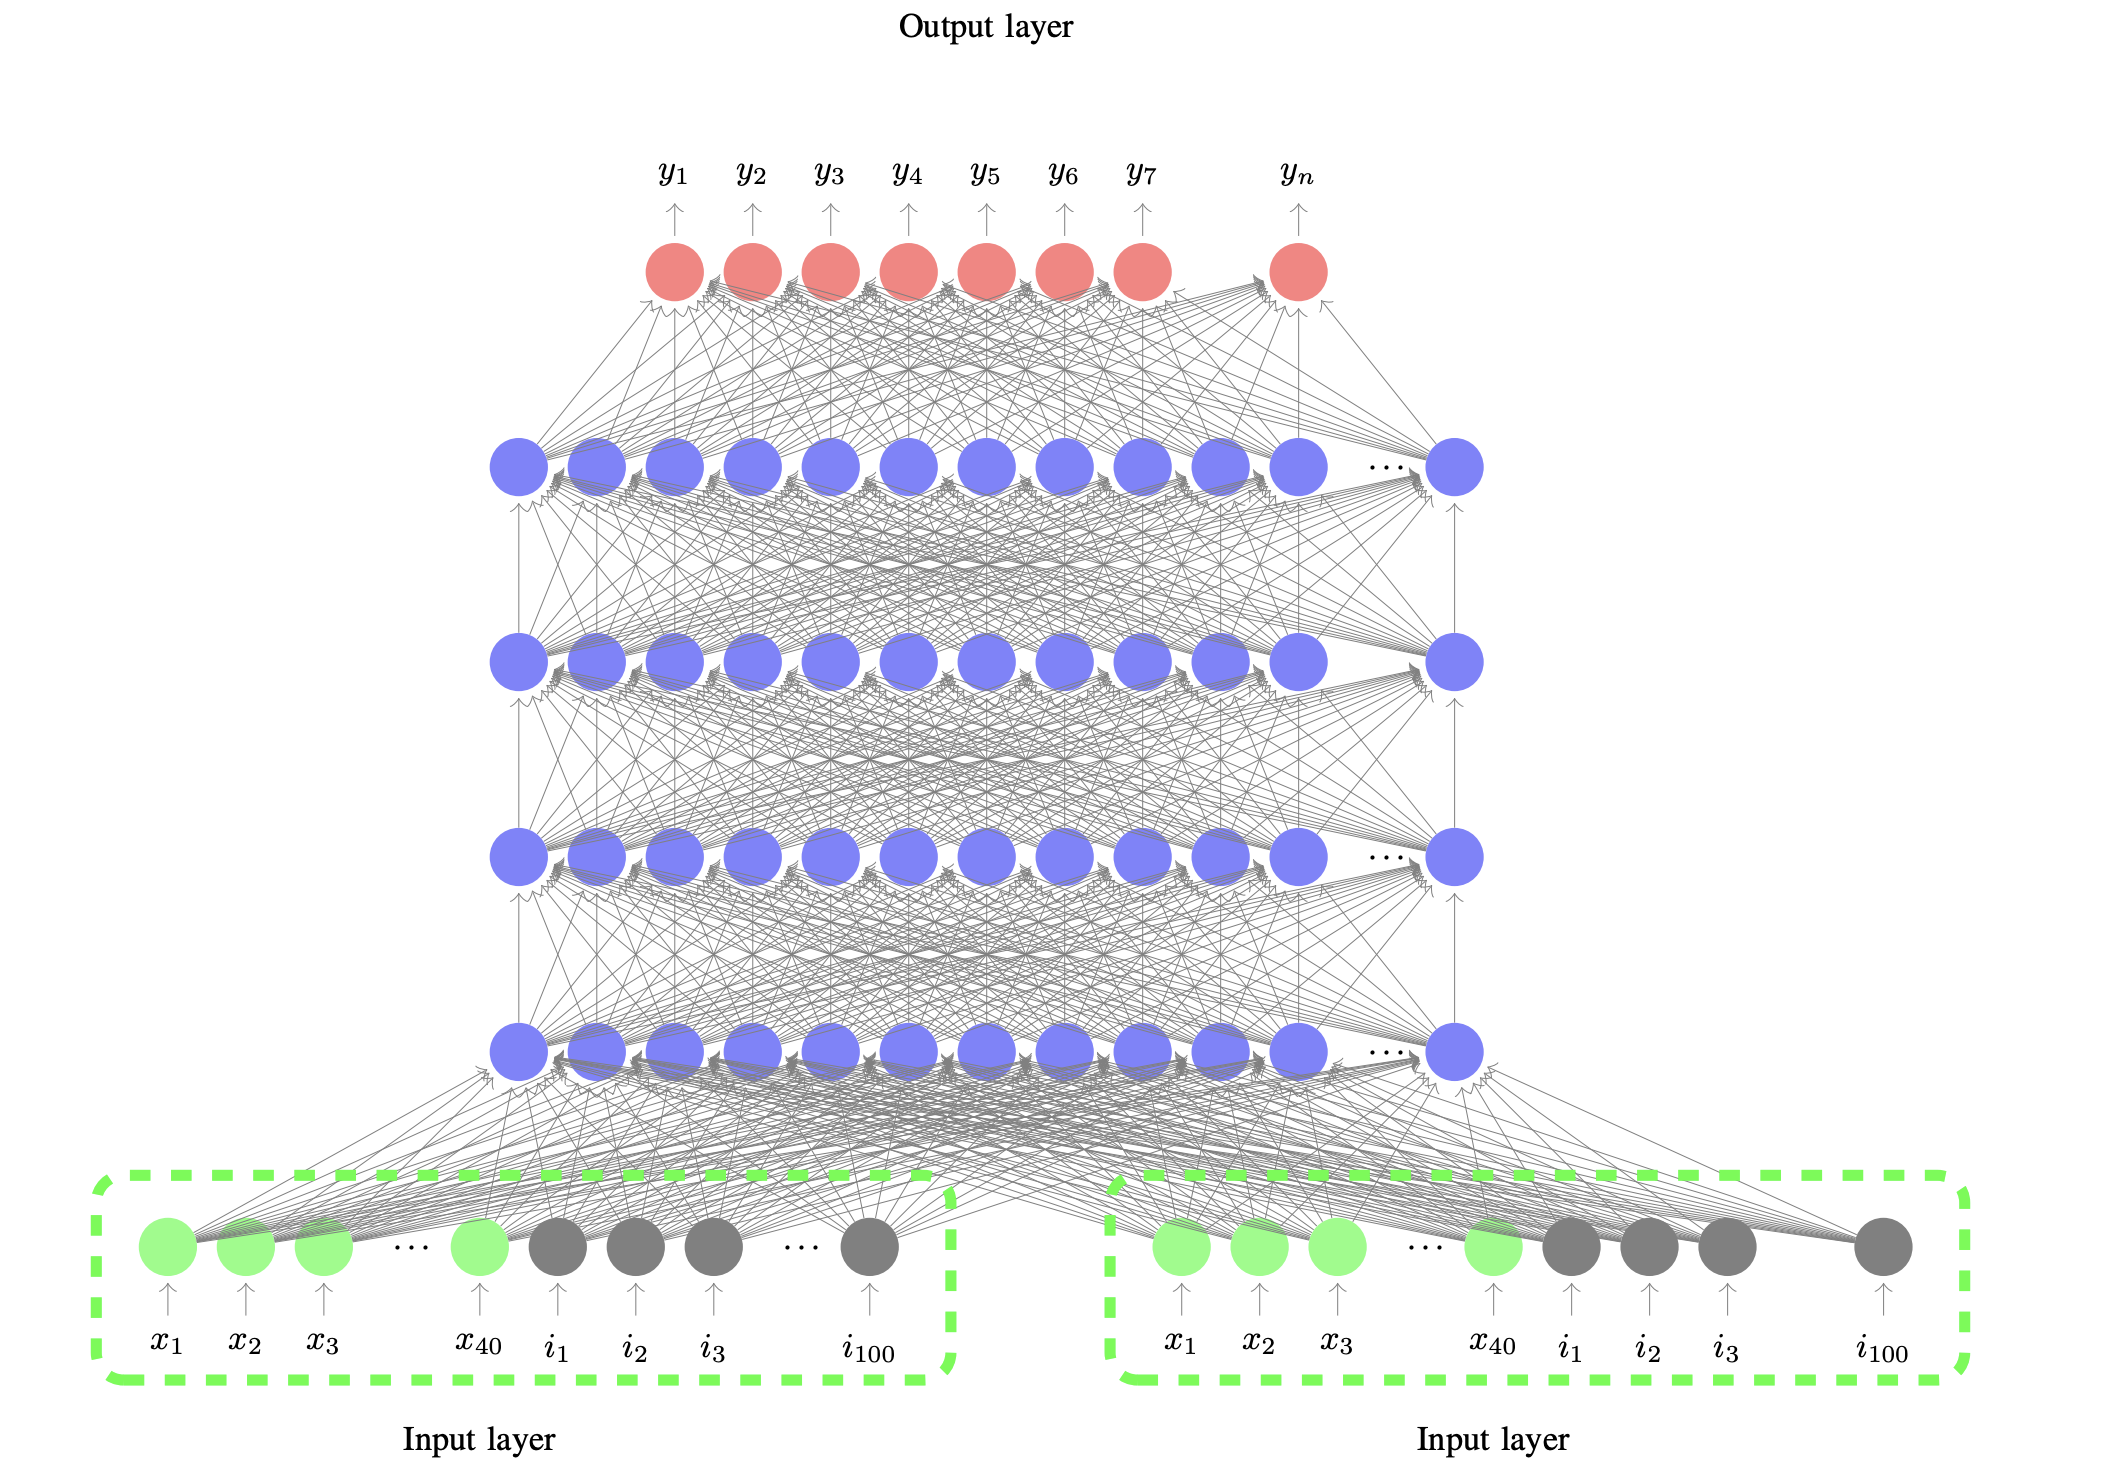
\includegraphics[width=0.48\textwidth]{imgs/tf_children.png}}
\subfigure[Pronunciation adaptation]{\label{fig:pronunciation_adapt}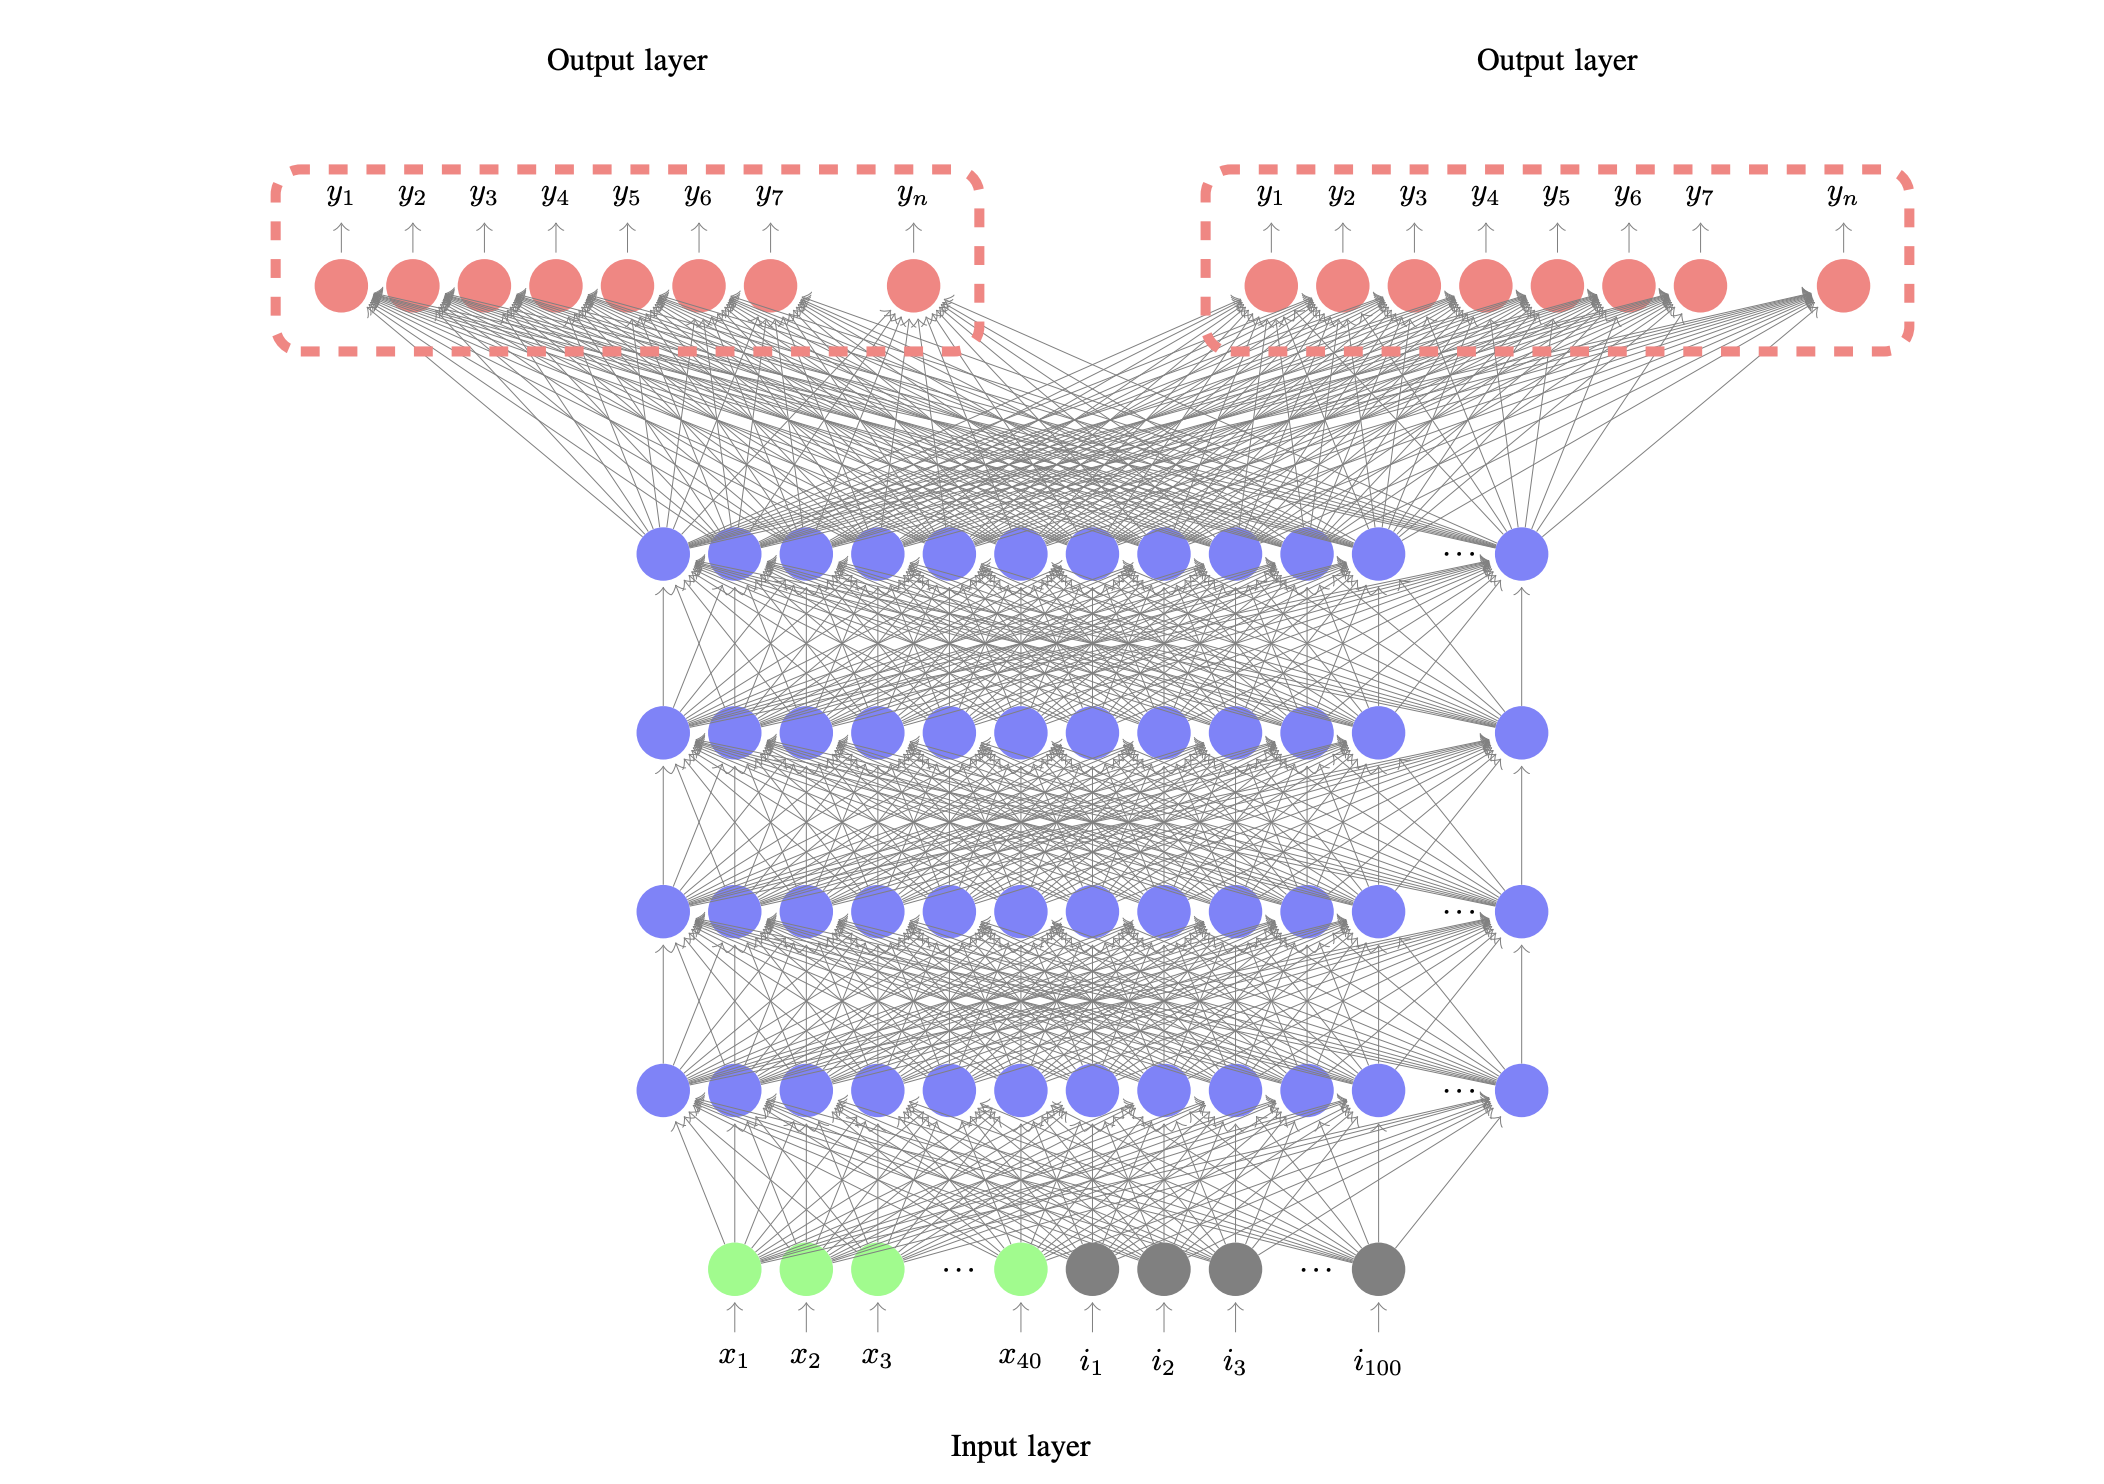
\includegraphics[width=0.48\textwidth]{imgs/pronunciation_adapt.png}}
\caption{Transfer learning approaches. Figures from \cite{TFchildren}}
\end{figure}

In recent years, \ac{TL} has emerged as a highly successful technique across various applications, particularly effective for low-resource tasks, in domains such as as language understanding \cite{Bert}, character recognition \cite{tfcharacter}, and dysarthric speech recognition \cite{tfpathology}, among others. The successes in these domains have motivated interest in exploring the utility of transfer learning for children's speech recognition. In particular, given the prevalence of large adult speech corpora, acoustic models trained on adult  are increasingly efficient and contain many acoustic and phonetic informations that can be used for efficient adaptation to children's speech. Since children's speech variabilities are present in both acoustics and linguistics, \cite{TFchildren} proposed investigating three distinct transfer learning methods to assess the contributions of acoustic adaptation, pronunciation adaptation, and their combination in the context of children's speech recognition.

% Acoustic adaptation
Acoustic adaptation targets the lower-level layers, leveraging the established notion that these layers capture acoustic properties. The methodology involves freezing the weights of the top-level layer and applying transfer learning to the lower-level layers, as depicted in Figure \ref{fig:acoustics_adapt}. In experiments conducted by \cite{TFchildren} and \cite{TransferLF}, acoustic transfer learning from an adult model to children's speech, by retraining only the first layers, yielded substantial relative \ac{WER} improvements of 38\% and 26\%, respectively, compared to the performance of adult models. Impressively, the acoustic adaptation outperformed a randomly initialised acoustic model trained on the same children's data, achieving a 4.9\% relative \ac{WER} improvement.

% Pronunciation adaptation
Pronunciation adaptation, based on the idea that higher-level layers capture task-specific information, focuses on adapting these layers while keeping lower-level layers frozen. As illustrated in Figure \ref{fig:pronunciation_adapt}, \cite{TFchildren} conducted experiments applying pronunciation adaptation to the last layers of the model, resulting in a significant 31\% relative \ac{WER} improvement compared to the performance of the adult model. However, when compared to a randomly initialised acoustic model trained with the same children's data, pronunciation adaptation degrades by 5.6\% relative \ac{WER}.

% Combination of acoustic and pronunciation / TL on all layers
In recent years,\ac{TL} has emerged as a highly successful technique across various applications, particularly proving effective in low-resource tasks such as language understanding \cite{Bert}, character recognition \cite{tfcharacter}, and dysarthric speech recognition \cite{tfpathology}, among others. The achievements in these domains have spurred interest in exploring the utility of transfer learning for children's speech recognition, a domain often characterised by limited labeled data.

Given the prevalence of large corpora derived from adult speech, recent acoustic models trained on adult data have demonstrated high efficiency and encapsulate rich acoustic and phonetic information. Motivated by these successes, \cite{TFchildren} proposed investigating three distinct transfer learning methods to assess the contributions of acoustic adaptation, pronunciation adaptation, and their combination in the context of children's speech recognition.

Acoustic adaptation targets the lower-level layers, leveraging the established notion that these layers capture acoustic properties. The methodology involves freezing the weights of the top-level layer and applying transfer learning to the lower-level layers, as depicted in Figure \ref{fig:acoustics_adapt}. In experiments conducted by \cite{TFchildren} and \cite{TransferLF}, acoustic transfer learning from an adult model to children's speech, by retraining only the first layers, yielded substantial relative \ac{WER} improvements of 38\% and 26\%, respectively, compared to the performance of adult models. Impressively, the acoustic adaptation outperformed a randomly initialised acoustic model trained on the same children's data, achieving a 4.9\% relative \ac{WER} improvement.

Pronunciation adaptation, premised on the idea that higher-level layers capture task-specific information, focuses on adapting these layers while keeping lower-level layers frozen. As illustrated in Figure \ref{fig:pronunciation_adapt}, \cite{TFchildren} conducted experiments applying pronunciation adaptation to the last layers of the model, resulting in a significant 31\% relative \ac{WER} improvement compared to the performance of the adult model. However, when compared to a randomly initialized acoustic model trained with the same children's data, pronunciation adaptation exhibited a 5.6\% relative \ac{WER} degradation.

Finally, the combination of acoustic and pronunciation adaptation, achieved through fine-tuning the entire network, demonstrated outperforms performances compared to individual adaptations. This aligns with recent observations in end-to-end models, where transfer learning from an adult pre-trained model outperformed training from scratch using only children's data only \cite{sri_end2end, gelin2021endtoend}. These findings underscore the efficacy of transfer learning strategies for optimising acoustic and pronunciation adaptation in children's \ac{ASR}. 

% Multi-task
\subsubsection{Multi-task learning}%************************************************************
\label{section:MTL}
\begin{figure}[t]
\begin{center}

\includegraphics[width=0.7\textwidth]{imgs/MTL.png}
\caption{Multilingual approach using each language as a task in a multi-task learning context.}
\label{fig:MTL}
\end{center}
\end{figure}

\ac{MTL}, like to transfer learning, draws inspiration from biological intelligence. In contrast to transfer learning, \ac{MTL} does not train solely on source and target tasks in a sequential manner, here \ac{MTL} simultaneously train on multiple tasks at the same time. The fundamental objective of \ac{MTL} is to discover shared representations among related tasks.  In general, a typical \ac{MTL} model consists of two distinct components. The first part is a sub-network shared by all tasks, while the second part consists of task-specific output sub-networks, as illustrated in Figure \ref{fig:MTL}. The shared layers facilitate the learning of a joint representation that is more robust, enhancing the model's reliability across diverse tasks.

More formally, for any task $i$ the corresponding output of the forward pass will be:
\begin{equation} \label{equation:MT}
    f(X_i;\{M_i, M_{c}\}) = f_i(f_{c}(X_i,{M_{c}}); {M_i}) 
\end{equation}
where $X_i$ is the data associated with the task $i$, $M_i$ represents the task-specific parameters of the model, and $M_{c}$ corresponds to the parameters that are shared (or common) across all tasks.

In consequence, the performances of \ac{MTL} is intricately tied to the degree of relatedness among tasks used during training. Indeed, its efficacy diminishes when confronted with outlier tasks that are unrelated to the majority of the other tasks. This sensitivity is due to the inherent challenge of learning common representations for tasks that lack substantial relatedness to one another \cite{zhang2018overview}. This task-relatedness consideration underscores the importance of thoughtful task selection when using \ac{MTL} techniques.

Moreover, \ac{MTL} has been used effectively in a variety of areas, including natural language processing \cite{multi-nlp}, computer vision \cite{mtl_computervision} and bioinformatics \cite{bioinfo}. \ac{MTL} has been naturally applied in the field of automatic speech recognition \cite{MTL-LFMMI} with directly application to low-resource \ac{ASR} \cite{abad2020}. Given that \ac{ASR} for children represents a resource-limited task, \ac{MTL} has been proposed as a strategy to mitigate the issue of data scarcity. Notably, studies such as \cite{TransferLF} and \cite{2019multi} successfully applied \ac{MTL} to Mandarin and English-speaking children, with a 16.96\% relative improvement in \ac{WER} for the English children.

%SSL
\subsubsection{Self-supervised Learning}
% First step is semi-supervised
A first step towards \ac{SSL} was the introduction of semi-supervised techniques, such as pseudo-labeling. Semi-supervised appraoches were a dominant training strategies for using unlabeled data. In particular, The pseudo-labeling starts with the training of a ``teacher" model on a set of supervised data. Subsequently, pseudo-labels are generated for unlabeled data by leveraging the predictions of the trained teacher model. Following this, a ``student" model is trained using a combined dataset comprising both supervised and pseudo-labeled data. Importantly, the pseudo-labeling process can be iteratively repeated multiple times to enhance the quality of teacher-generated labels \cite{zavaliagkos1998utilizing,ma2006unsupervised}. It is noteworthy that, as of today, some of the most effective \ac{ASR} models, such as the Whisper model, leverages pseudo-labeling as a crucial component of its training strategy \cite{radford2023robust}. However, the performances of semi-supervised, and particularly pseudo-labeling, has been found to be highly dependent on the quality of the teacher model, prompting the need for more robust and sophisticated training strategies.

% Then comes SSL
In this context, \ac{SSL} has emerged as a paradigm designed to acquire general data representations direclty from unlabeled examples, subsequently allowing transfer learning on a small amount of labeled data. This approach has proven particularly successful in the domain of natural language processing \cite{sarzynska2021detecting} and computer vision \cite{henaff2020data}.
% PASE features
One notable first attempt to bring \ac{SSL} to the speech domain was made by the introduction of the \ac{PASE} and its extension,\ac{PASE}+. These innovations demonstrated the capability to learn meaningful speech information such as speaker identities, phonemes, and emotions. The \ac{PASE} framework operates by encoding raw speech waveforms into a representation, which is then input to multiple regressors and discriminators. The regressors within \ac{PASE} are standard features computed from the input waveform. While the discriminators focus on positive or negative samples and are trained to effectively separate them. Both the regressors and discriminators play a crucial role in incorporating prior knowledge into the encoder, a key factor for deriving meaningful and robust representations. 

% Wav2vec2 and Hubert
Recently, self-supervised systems have obtained remarkable results with the introduction of models employing \ac{BERT}-like training methodologies, such as Wav2vec2 \cite{baevski2020wav2vec} and HuBERT \cite{hsu2021hubert}. Notably, the success of these models can be attributed to the conjunction use of masking, discrete speech units, contextualized representations, and contrastive loss. The integration of masking techniques allows these models to effectively learn contextualised representations by masking certain portions of the input data and predicting them based on the remaining context. The use of discrete speech units enable the model to be more robust to variations, while the contrastive loss functions enhances the discriminative power of these models by encouraging the model to differentiate between positive and negative samples.
% SSL for children
Motivated by the successes of \ac{SSL} methods in overcoming challenges in low-resource \ac{ASR} tasks, such as low-resource languages \cite{riviere2020unsupervised}, noisy speech \cite{wang2022wav2vec}, and accented speech \cite{li2021accent}, the integration of \ac{SSL} for children's \ac{ASR} marked its debut in 2021, with a first place in a non-native children's speech recognition challenge \cite{xu2021tal}. Subsequent to this notable success, the application of \ac{SSL} for children's \ac{ASR} has gained increased attention, especially with the use of models like Wav2vec2 \cite{jain2023wav2vec2,jain2023adaptation,fan2022draft}. A concise analysis of various \ac{SSL} approaches as frozen feature extractor for children's \ac{ASR} has been conducted within the context of this thesis, and the findings are presented in Annex \ref{chapter:appendixB}.
   
\section{Children Corpora}
\label{section:children_corpora}
As described in Chapter \ref{section:data_scarcity}, notwithstanding recent efforts to assemble dedicated databases for children's speech, the quantity of available data remains lower compared to that for adults. Collecting speech data from children  is challenging in many ways, from factors such as limited attention spans, frequent mispronunciations, ungrammatical expressions, and the use of non-standard vocabulary. These difficulties involved in capturing high-quality child speech data contribute to the scarcity of publicly accessible child speech corpora. The relatively modest sizes of these datasets present obstacles to research efforts and impede progress in developing reliable \ac{ASR} systems for children.


\begin{table}
%\centering
\small
\begin{tabular}{l|c|c|c|c|c|c} 
\hline
\multicolumn{1}{c|}{\textbf{Corpus}} & \multicolumn{1}{c|}{\textbf{Languages}} & \multicolumn{1}{c|}{\textbf{\# Spkrs}} & \multicolumn{1}{c|}{\textbf{\# Utt}} & \multicolumn{1}{c|}{\textbf{Dur.}} & \multicolumn{1}{c|}{\textbf{Age Range}} & \multicolumn{1}{c}{\textbf{Date}} \\ 
\hline
Providence Corpus \cite{providence} & English & 6 &  & 363h & 1-3 & 2006 \\ 
\hline
Lyon Corpus \cite{LyonSC} & French & 4 &  & 185h & 1-3 & 2007 \\ 
\hline
CASS\_CHILD \cite{cass_child} & Mandarin & 23 &  & 631h & 1-4 & 2012 \\ 
\hline
Demuth Sesotho Corpus \cite{demuth1992acquisition} & Sesotho & 4 & 13250 & 98h & 2-4 & 1992 \\ 
\hline
NITK Kids’ Speech Corpus \cite{nitk} & Kannada & 160 &  & 10h & 2-6 & 2019 \\ 
\hline
CHIEDE \cite{chiede} & Spanish & 59 & 15,444 & 8h & 3-6 & 2008 \\ 
\hline
CUChild \cite{cuchild} & Cantonese & 1,986 &  &  & 3-6 & 2020 \\ 
\hline
EmoChildRu \cite{emochildru} & Russian & 100 & 20,000 & 30h & 3-7 & 2015 \\ 
\hline
CNG Portuguese children\cite{hamalainen2013cng} & Portuguese & 510 &  & 21h & 3-10 & 2013 \\ 
\hline
AusKidTalk$^1$ \cite{ahmed2021auskidtalk} & English & 750 &  & 600h & 3-12 & 2021 \\ 
\hline
UCLA JIBO kids \cite{yeung2019robotic} & English & 130 &  &  & 4-7 & 2019 \\ 
\hline
\textbf{PF-STAR-SWEDISH} \cite{pfstar}
& Swedish & 198 & 8,909 & 6h & 4-8 & 2005 \\ 
\hline
SLT 2021 \cite{yu2021slt} & Mandarin & 981 &  & 58h & 4-11 & 2021 \\ 
\hline
PF-STAR Children British \cite{pfstar,russell2006pf,pf-star-british} & English & 158 &  & 14.5h & 4-14 & 2006 \\ 
\hline
AD-child. RU \cite{ad-child_ru} & Russian & 278 &  &  & 4-16 & 2019 \\ 
\hline
TBALL \cite{tball} & English & 256 & 5,000 & 40h & 5-8 & 2005 \\ 
\hline
SPECO \cite{speco} & Hungarian & 72 &  & 12h & 5-11 & 1999 \\ 
\hline
UltraSuite\cite{eshky2019ultrasuite} & English & 86 & 14,456 & 37h & 5-14 & 2019 \\ 
\hline
CID read speech corpus \cite{lee1999acoustics} & English & 436 &  &  & 5-18 & 1996 \\ 
\hline
Persian Kids Speech Corpus \cite{khanzadi2022persian} & Persian & 286 & 162,395 & 33h & 6-9 & 2022 \\ 
\hline
\textbf{Letsread$^2$} \cite{letsread} & Portuguese & 284 & 4,629 & 14h & 6-10 & 2016 \\ 
\hline
\textbf{CMU kids Corpus} \cite{cmu} & English & 76 & 5,180 &  & 6-11 & 1997 \\ 
\hline
CFSC \cite{CFSC} & Filipino & 57 &  & 8h & 6-11 & 2012 \\ 
\hline
IESC-Child \cite{PEREZESPINOSA202055} & Spanish & 174 & 19,793 & 34h & 6-11 & 2020 \\ 
\hline

CU Children's read and prompted \cite{hagen2003children}& English & 663 & 66300 &  & K-G5 & 2001 \\ 
\hline
\textbf{Chorec$^2$} \cite{chorec} & Dutch & 400 & 3,065 & 25h & 6-12 & 2008 \\ 
\hline
ChildIt2 \cite{childit2} & Italian & 96 &  4,875 & 9h & 6-14 & 2016 \\ 
\hline
TIDIGITS \cite{leonard1993tidigits} & English & 101 &  &  & 6-15 & 1993 \\ 
\hline
CSLU Kids' Speech Corpus \cite{cslu} & English & 1,100 & 1,017 &  & K-G10 & 2007 \\ 
\hline
SingaKids-Mandarin \cite{singakids} & Mandarin & 255 & 79,843 & 125h & 7-12 & 2016 \\ 
\hline
ChildIt corpus \cite{gerosa2006acoustic} & Italian & 171 &  &  & 7-13 & 2007 \\ 
\hline
VoiceClass Database \cite{burkhardt2010database} & German & 170 &  &  & 7-14 & 2010 \\ 
\hline
Deutsche Telekom telephone \cite{burkhardt2010database} & German & 106 &  &  & 7-14 & 2010 \\ 
\hline
Jasmin \cite{JASMIN} & Dutch &  &  & 63h & 7-16 & 2008 \\ 
\hline
Tgr-child corpus \cite{gerosa2006acoustic} & Italian & 30 &  &  & 8-12 & 2007 \\ 
\hline
SponIt corpus \cite{gerosa2006acoustic} & Italian & 21 &  &  & 8-12 & 2007 \\ 
\hline
Swedish NICE Corpus \cite{bell2005swedish} & Swedish & 75 & 5,580 &  & 8-15 & 2005 \\
\hline
CHIMP spontaneous speech \cite{language_children2} & English & 160 &  &  & 8-14 & 2002 \\ 
\hline
SpeeCon corpus  \cite{SPEECONS} & 20 Languages &  &  &  & 8-15 & 2002 \\ 
\hline
Rafael.0 telephone corpus \cite{linguistic-children} & Danish & 306 &  &  & 8-18 & 1996 \\ 
\hline
\textbf{Boulder Learning - MyST} \cite{MyST} & English & 1,371 & 228,874 & 384h & G3-G5 & 2019 \\ 
\hline
CU Story Corpus \cite{hagen2003children} & English & 106 & 5,000 & 40h & G3-G5 & 2003 \\ 
\hline
\textbf{ETLT$^2$} \cite{etlt} & L2 German &  & 1,674 & 6h & 9-16 & 2020 \\ 
\hline
Lesetest corpus \cite{grissemann2000zurcher} & German & 62 &  &  & 10-12 & 2000 \\ 
\hline
FAU Aibo Emotion Corpus \cite{steidl2009automatic} & German & 51 & 13,642 & 9h & 10-13 & 2002 \\ 
\hline
PIXIE corpus \cite{bell2003child} & Swedish & 2,885 &  &  &  & 2003 \\ 
\hline
Takemaru-kun corpus \cite{takemaru} & Japanese & 17,392 &  &  & & 2007 \\ 
\hline
CALL-SLT \cite{callslt} & German &  & 5,000 &  &  & 2014 \\ 
\hline
\multicolumn{7}{l}{$^1$ To this day, data collection for this dataset is not complete.} \\
\multicolumn{7}{l}{$^2$ Information displayed here correspond to a subset of the original data used in this proposal.}  \\
\end{tabular}
\caption{Non-exhaustive comparison of children's speech corpora. This table has been sorted by age range. Blanks indicate unavailable information. Entries highlighted in bold correspond to the corpora used in the experiments presented in this thesis. K: Kindergarden. G: Grade}
\label{table:children_corpora}
\end{table}

Table \ref{table:children_corpora} presents a compilation of existing corpora of children's speech. Notably, approximately one-third of the available corpora are in English. Likewise, a comparable proportion is specifically oriented towards children under the age of 4. It is crucial to acknowledge the inherent trade-offs in these corpora, involving considerations of speaker diversity, total duration, and the number of utterances.

Subsequently, the remainder of this section will go through an examination of the children's speech corpora employed in this thesis.


\subsection{LETSREAD}
LetsRead database \cite{letsread} is a read-aloud speech database of European Portuguese from children aged 6 to 10,  from 1st to 4th grade. This corpus is composed of a total of 284 children, 147 girls and 137 boys, whose mother tongue is European Portuguese. Children from private and public Portuguese schools were asked to carry out two tasks: reading sentences and a list of pseudo-words. The difficulty of the tasks varies depending on the school year of the child. 
For this proposal, we excluded all utterances from the pseudo-word reading task because we do not include pseudo-words in the language model and lexicon in our experiments. 
\subsection{PFSTAR\_SWEDISH}
The PFStar children's speech corpus \cite{pfstar} was collected as part of the EU FP5 PFSTAR project. It contains more than 60 hours of speech. This corpus is divided into two parts: native-language speech and non-native language part.
The native-language speech part contains recordings of British English, German and Swedish children, from 4 to 14 years old. The non-native language part consists of speech by Italian, German and Swedish children speaking English. In this work, we only used the native language Swedish part, consisting of speech by 198 native Swedish children, between 4 and 8 years old recorded in the Stockholm area, imitating an adult who read the text from a screen.
\subsection{ETLTDE}
\ac{ETLT} corpus \cite{etlt} has been collected in northern Italy for assessing English and German proficiency of Italian children between 9 and 16 years old, by asking them to answer questions. The data collection was carried out in schools. On average the signal quality is good, but some background noise is often present (doors, steps, keyboard typing, background voices, street noises if the windows are open, etc). In addition, many answers are whispered and difficult to understand.
For this thesis, we only used the German-transcribed subset ,named ETLTDE , a subset containing around 6 hours of speech divided into training and test partitions.
\subsection{CMU\_KIDS}
The \ac{CMU} kids corpus \cite{cmu} contains English sentences read aloud by children, 24 males and 52 females, from 6 to 11 years old. In total, 5,180 utterances were recorded with one sentence per utterance. This database was created to train the SPHINX II \cite{sphinx2} automatic speech recognition system within the LISTEN project at \ac{CMU}.
\subsection{CHOREC}
\label{subsection:chorec}
The Chorec corpus \cite{chorec} consists of 400 Dutch-speaking elementary school children, between 6 and 12 years old, reading words, pseudo-words and stories. The difficulty of the reading task was adapted to children with 9 different levels. Recordings were made in schools, leading to some environmental noises (school bells, children entering the playground etc.). For this thesis, similarly to the LETSREAD dataset, we discarded pseudo-word utterances.

\subsection{MyST}
\ac{MyST} Children Speech Corpus \cite{MyST} is currently one of the largest publicly available corpora of English children's speech, with around 400 hours. This is about 10 times more than all other English children's speech corpora combined. It consists of conversations between children and a virtual tutor in 8 scientific domains. Speech was collected from 1,372  students in third, fourth and fifth grades. Partitioning of the corpus is already available, ensuring reasonably representation of each scientific domain and that each student is present in only one partition. However, only 45\% of the utterances were transcribed at the word level. Furthermore, for the purposes of this thesis, we decided to remove all utterances shorter than one second and longer than 30 seconds. After this filtering, 81971 utterances from 736 speakers for a total of 151 hours remain.


\section{Summary}
In this chapter, we provided an overview of children's \ac{ASR}, its inherent challenges, and the ongoing responses from the research community. The complexity of \ac{ASR} in children arises primarily from the developmental nuances of the vocal apparatus, resulting in an acoustic mismatch with adult speech, although this mismatch gradually diminishes until around the age of 15. Despite sustained efforts, \ac{ASR} for children remains ctive and challenging area of research.

Our examination in this chapter highlights that knowledge transfer approaches, such as transfer learning and multi-task learning, appear to be promising avenues for improving children's \ac{ASR}. Additionally, the exploration of synthetic speech generation, using \ac{TTS} systems, has captured our attention as a potential strategy for improvement. These methodologies will be applied and explored in-depth in the subsequent chapters of this thesis.

Moreover, we have presented a comprehensive comparison of children's speech corpora, which, to the best of our knowledge, stands as the most exhaustive compilation available. This analysis provides valuable insights into the landscape of available datasets for children's speech.
